\documentclass[13pt,oneside]{scrbook}
\usepackage{tocloft,calc}
\pagestyle{plain}
\usepackage{times}
\usepackage[english,vietnam]{babel}
\usepackage[utf8]{inputenc}
\usepackage{url}
%% Thêm chữ Chương vào mục lục
\renewcommand{\cftchappresnum}{Chương }
\AtBeginDocument{\addtolength\cftchapnumwidth{\widthof{\bfseries Chương }}}
\renewcommand{\cfttoctitlefont}{\normalfont\hfill\Large\bfseries\MakeUppercase}
\renewcommand{\cftaftertoctitle}{\hfill} %two lines above together give a centered Large bold title
\renewcommand{\cftchapfont}{\bfseries}
\renewcommand\cftchapaftersnum{.}% adds dot after chapter title in ToC
%% End Thêm chữ Chương vào mục lục
%% CHƯƠNG và tên chương cùng một dòng
%%Table
\newcounter{magicrownumbers}
\newcommand\rownumber{\stepcounter{magicrownumbers}\arabic{magicrownumbers}}
%% End Table
\usepackage{titlesec}
\titleformat{\chapter}[hang] 
{\normalfont\Large\bfseries}{\MakeUppercase{\chaptertitlename}\ \thechapter.}{1em}{\MakeUppercase} 
\titlespacing*{\chapter}{0cm}{-30pt}{14pt}[0pt]
%% Chương và tên chương cùng một dòng
\def\@biblabel#1{\def\citename##1{##1}[#1]\hfill}
\usepackage{lipsum}
\titleformat{\section}
  {\normalfont\fontsize{14}{15}\bfseries}{\thesection}{1em}{\MakeUppercase}
\titleformat{\subsection}
  {\normalfont\fontsize{14}{15}\bfseries}{\thesubsection}{1em}{}
\titleformat{\subsubsection}
  {\normalfont\fontsize{14}{15}\bfseries}{\thesubsubsection}{1em}{}
\usepackage{mathrsfs}
\usepackage{upgreek}
\usepackage{amsmath}
\usepackage{empheq}
\usepackage{amsfonts}
\usepackage{amssymb}
\usepackage{scrextend}
\usepackage{a4wide,amssymb,epsfig,latexsym,multicol,array,hhline,fancyhdr}
\usepackage{lastpage}
\usepackage{enumerate}
\usepackage{color}
\usepackage{graphicx}
\usepackage{array}
\usepackage{tabularx}
%% --- Reset Row Table Row Number to 0
\usepackage{etoolbox}
\preto\tabular{\setcounter{magicrownumbers}{0}}
%% --- End Reset Row Table Row Number to 0
\usepackage{multirow}
\usepackage{multicol}
\usepackage{rotating}
\usepackage{url}
\usepackage{graphics}
\usepackage{geometry}
\usepackage[table]{xcolor}
\geometry{
	a4paper,
	total={210mm,297mm},
	left=30mm,
	right=30mm,
	top=20mm,
	bottom=20mm,
}
\usepackage{setspace}
\usepackage{epsfig}
\usepackage{tikz}
\usetikzlibrary{calc}
\usepackage{booktabs}
\usepackage{footnote}
\usepackage{makecell}
\usetikzlibrary{shapes,arrows,arrows,snakes,backgrounds}

\newtheorem{theorem}{{\bf Theorem}}
\newtheorem{property}{{\bf Property}}
\newtheorem{proposition}{{\bf Proposition}}
\newtheorem{corollary}[proposition]{{\bf Corollary}}

%Strecth line 1.3
\renewcommand{\baselinestretch}{1.3}
\renewcommand{\UrlFont}{\small\tt}
%% Algorithm
\usepackage{algpseudocode,algorithm,algorithmicx}
\usepackage{caption}% http://ctan.org/pkg/caption
%\setlength{\belowcaptionskip}{-30pt} % khoach cach tu ten hinh toi van ban ben duoi
%\usepackage{float}
\setlength{\floatsep}{4pt plus 0pt minus 0pt}
\setlength{\textfloatsep}{4pt plus 0pt minus 0pt}
\setlength{\intextsep}{4pt plus 0pt minus 0pt}

\captionsetup[ruled]{labelsep=period}
\newcommand*\Let[2]{\State #1 $\gets$ #2}
\algrenewcommand\algorithmicrequire{\textbf{Precondition:}}
\algrenewcommand\algorithmicensure{\textbf{Postcondition:}}
\let\emptyset\varnothing
%\floatname{algorithm}{Giải thuật}
\setlength{\dbltextfloatsep}{0pt}
%% End Algorithm
\usepackage{cases}
\newcommand\specialchapter{%
  \titleformat*{\chapter}{\centering}
}
\newcommand\normalchapter{%
\titleformat{\chapter}[hang] 
{\normalfont\Large\bfseries}{\MakeUppercase{\chaptertitlename}\ \thechapter.}{1em}{\MakeUppercase} 
}
%% Create link for table of content
\usepackage{hyperref}
\hypersetup{
    colorlinks,
    linkcolor={black!50!black},
    citecolor={black!50!black},
    urlcolor={black!80!black}
}
\begin{document}
% Trang bia trong
\newpage
\begin{titlepage}
	\begin{tikzpicture}[remember picture, overlay]
	\draw [line width=3pt]
	($ (current page.north west) + (2.0cm,-2.0cm) $)
	rectangle
	($ (current page.south east) + (-1.5cm,1.8cm) $);
	\draw [line width=1pt]
	($ (current page.north west) + (2.15cm,-2.15cm) $)
	rectangle
	($ (current page.south east) + (-1.65cm,1.95cm) $); 
	\end{tikzpicture}
	\begin{center}
		{\fontsize{12}{12}\selectfont \textbf{ĐẠI HỌC QUỐC GIA TP. HỒ CHÍ MINH}}\\
		\vspace{0.3cm}
		{\fontsize{14}{12}\selectfont \textbf{TRƯỜNG ĐẠI HỌC BÁCH KHOA}}\\
		\noindent\rule{5cm}{0.5pt}\\
		\begin{figure}[h!]
			\begin{center}	
				
\includegraphics[width=30mm]{hcmut.png}
			\end{center}
		\end{figure}
		\vspace{0.5cm}
		{\fontsize{16}{12}\selectfont \textbf{NGUYỄN VĂN DƯƠNG}}\\
		\vspace{2cm}
		{\fontsize{18}{24}\selectfont \textbf{SO SÁNH HAI PHƯƠNG PHÁP THU GỌN TẬP HUẤN LUYỆN RHC VÀ NAIVE RANKING TRONG PHÂN LỚP DỮ LỆU CHUỖI THỜI GIAN}}\\
		\vspace{2cm}
		{\fontsize{18}{22}\selectfont \textbf{LUẬN VĂN THẠC SĨ}}\\			
		\vspace{6.5cm}
		{\fontsize{12}{12}\selectfont TP. HỒ CHÍ MINH - 2018}\\	
	\end{center}
\end{titlepage}
% Trang bia trong	
\newpage
\begin{titlepage}
	\begin{tikzpicture}[remember picture, overlay]
	\draw [line width=3pt]
	($ (current page.north west) + (2.0cm,-2.0cm) $)
	rectangle
	($ (current page.south east) + (-1.5cm,1.8cm) $);
	\draw [line width=1pt]
	($ (current page.north west) + (2.15cm,-2.15cm) $)
	rectangle
	($ (current page.south east) + (-1.65cm,1.95cm) $); 
	\end{tikzpicture}
	\begin{center}
	{\fontsize{12}{12}\selectfont \textbf{ĐẠI HỌC QUỐC GIA TP. HỒ CHÍ MINH}}\\
	\vspace{0.3cm}
	{\fontsize{14}{12}\selectfont \textbf{TRƯỜNG ĐẠI HỌC BÁCH KHOA}}\\
	\noindent\rule{5cm}{0.5pt}\\
	\begin{figure}[h!]
	\begin{center}	
	
\includegraphics[width=30mm]{hcmut.png}
	\end{center}
	\end{figure}
	\vspace{0.5cm}
	{\fontsize{16}{12}\selectfont \textbf{NGUYỄN VĂN DƯƠNG}}\\
	\vspace{2cm}
	{\fontsize{18}{22}\selectfont \textbf{SO SÁNH HAI PHƯƠNG PHÁP THU GỌN TẬP HUẤN LUYỆN RHC VÀ NAIVE RANKING TRONG PHÂN LỚP DỮ LỆU CHUỖI THỜI GIAN}}\\
	\vspace{0.5cm}
	{\fontsize{12}{22}\selectfont CHUYÊN NGÀNH: KHOA HỌC MÁY TÍNH}\\	
	{\fontsize{12}{22}\selectfont MÃ SỐ CHUYÊN NGÀNH: 60.48.01}\\
	\vspace{1cm}
	{\fontsize{18}{22}\selectfont \textbf{LUẬN VĂN THẠC SĨ}}\\
	\vspace{2cm}
	{\fontsize{12}{22}\selectfont \textbf{PGS. TS. DƯƠNG TUẤN ANH
}}\\
	\vspace{3.5cm}
	{\fontsize{12}{12}\selectfont TP. HỒ CHÍ MINH - 2018}\\	
	\end{center}
\end{titlepage}
\newpage
\begin{titlepage}
	\begin{tikzpicture}[remember picture, overlay]
	\draw [line width=1pt]
	($ (current page.north west) + (2.15cm,-2.15cm) $)
	rectangle
	($ (current page.south east) + (-1.65cm,1.95cm) $); 
	\end{tikzpicture}
	\begin{center}
	CÔNG TRÌNH ĐƯỢC HOÀN THÀNH TẠI \\TRƯỜNG ĐẠI HỌC BÁCH KHOA – ĐHQG - HCM\\
	\end{center}
Cán bộ hướng dẫn khoa học: PGS. TS. Dương Tuấn Anh\\
\\
Cán bộ chấm nhận xét 1: ....................................................\\
\\
Cán bộ chấm nhận xét 2: ....................................................\\
\\
Luận văn thạc sĩ được bảo vệ tại Trường Đại Học Bách Khoa, ĐHQG Tp.HCM vào ngày ..... tháng ..... năm 2018\\
Thành phần hội đồng đánh giá luận văn thạc sĩ gồm:
\begin{enumerate}
\item Chủ tịch: .........................................................
\item Phản biện 1: ....................................................
\item Phản biện 2: ....................................................
\item Uỷ viên: ...........................................................
\item Thư ký: ...........................................................
\end{enumerate}
Xác nhận của Chủ tịch Hội đồng đánh giá LV và Trưởng Khoa quản lý chuyên ngành sau khi luận văn được sửa chữa (nếu có)\\
\begin{center}
\textbf{CHỦ TỊCH HỘI ĐỒNG} \hspace{40mm} \textbf{TRƯỞNG KHOA}	
\end{center}
\end{titlepage}

\newpage
\begin{titlepage}

\begin{tabular}{c c}

\small ĐẠI HỌC QUỐC GIA TP.HCM & \small \textbf{CỘNG HÒA XÃ HỘI CHỦ NGHĨA VIỆT NAM}\\
\textbf{TRƯỜNG ĐẠI HỌC BÁCH KHOA}& \textbf{Độc lập - Tự do - Hạnh phúc}\\
--------------------------& ---------------------------
\end{tabular}

\vspace{1cm}
\centerline{\Large \textbf{NHIỆM VỤ LUẬN VĂN THẠC SĨ}}
\vspace{1cm}
\begin{tabular}{p{7cm} p{4cm}}
Họ tên học viên: \textbf{Nguyễn Văn Dương} & MSHV: \textbf{7140225} \\
Ngày, tháng, năm sinh: \textbf{06/11/1988} & Nơi sinh: \textbf{Vĩnh Long} \\
Chuyên ngành: Khoa học máy tính & Mã số: 60.48.01\\
\end{tabular}\\\\
\textbf{I. TÊN ĐỀ TÀI:}

So sánh hai phương pháp thu gọn tập huấn luyện RHC và Naive Ranking trong phân lớp dữ liệu chuỗi thời gian\\
\hspace{1cm} \textbf{II. NHIỆM VỤ VÀ NỘI DUNG}

\textbf{Nhiệm vụ}: Đề xuất giải thuật học chuyển đổi để hỗ trợ gom cụm gia tăng trong lĩnh vực giáo dục.

\textbf{Nội dung}:
\begin{enumerate}
\item Nghiên cứu lý thuyết về giải thuật phân lớp k-NN và các kỹ thuật thu gọn tập huấn luyện Naive Ranking, RHC, dRHC.
\item Hiện thực giải thuật phân lớp k-NN và các kỹ thuật thu gọn tập huấn luyện Naive Ranking, RHC, dRHC.
\item Thực nghiệm và so sánh kết quả phân lớp k-NN thuần tuý và phân lớp có kết hợp các kỹ thuật thu gọn tập huấn luyện Naive Ranking, RHC, dRHC.

\end{enumerate}
\textbf{III. NGÀY GIAO NHIỆM VỤ:} 26/02/2018 \\
\textbf{IV. NGÀY HOÀN THÀNH NHIỆM VỤ:} 17/06/2018 \\
\textbf{V. CÁN BỘ HƯỚNG DẪN:} PGS. TS. Dương Tuấn Anh \\\\
\begin{tabular}{c p{2cm} c}
 & &Tp.HCM, ngày ... tháng ... năm 2018\\
\textbf{CÁN BỘ HƯỚNG DẪN}& & \textbf{CHỦ NHIỆM BỘ MÔN ĐÀO TẠO}\\
\tiny (Họ tên và chữ ký) & & \tiny (Họ tên và chữ ký)\\

\end{tabular}

\vspace{0.5cm}
\centerline {\textbf{TRƯỞNG KHOA}}
\centerline {\tiny (Họ tên và chữ ký)}

\end{titlepage}

\newpage
% Thay doi theo format do trường quy định
\newgeometry{left=30mm,	right=20mm,	top=20mm, bottom=20mm}
\newpage
\thispagestyle{empty}
\pagenumbering{arabic}
\setcounter{page}{1}
\setlength{\footskip}{40pt} %Khoang cach tu noi dung trang den so trang
\pagenumbering{roman}
\setlength{\cftbeforetoctitleskip}{-0mm} %Reduce the space/gap from the top of the page to the table of contents title

\setcounter{tocdepth}{5}
\setcounter{secnumdepth}{4}
\pagenumbering{roman}

\specialchapter
\chapter*{LỜI CẢM ƠN}
\addcontentsline{toc}{chapter}{LỜI CẢM ƠN}
\newpage

\chapter*{TÓM TẮT LUẬN VĂN}
\addcontentsline{toc}{chapter}{TÓM TẮT LUẬN VĂN}
\newpage

\chapter*{ABSTRACT}
\addcontentsline{toc}{chapter}{ABSTRACT}
\newpage

\chapter*{LỜI CAM ĐOAN}
\addcontentsline{toc}{chapter}{LỜI CAM ĐOAN}
\newpage
\tableofcontents %summary insertion
\clearpage
\newpage

\chapter*{DANH MỤC HÌNH}
\addcontentsline{toc}{chapter}{DANH MỤC HÌNH}
%% Remove header of listoffigures
{\makeatletter
\let\@cftmakeloftitle\relax
\listoffigures% Print List of Figures
\makeatother}
\newpage

\chapter*{DANH MỤC BẢNG BIỂU}
\addcontentsline{toc}{chapter}{DANH MỤC BẢNG BIỂU}
\listoftables
\newpage

\chapter*{BẢNG THUẬT NGỮ ANH - VIỆT VÀ TỪ VIẾT TẮT}
\addcontentsline{toc}{chapter}{BẢNG THUẬT NGỮ ANH - VIỆT VÀ TỪ VIẾT TẮT}
\newpage

% % % % % % %
\normalchapter
\pagenumbering{arabic}
\setcounter{page}{1}
\chapter{GIỚI THIỆU ĐỀ TÀI}\label{Sec:Phan1}
\section{LÝ DO NGHIÊN CỨU}
Khai phá dữ liệu (hay còn gọi là khám phá tri thức hoặc dữ liệu) đã trở thành
lĩnh vực ngày càng quan trọng vì nó giúp phân tích và tổng kết dữ liệu thành những thông tin hữu ích. 
Có nhiều kỹ thuật trong quá trình khai thác dữ liệu trong đó \textit{phân lớp} (classification) được biết đến như một kỹ thuật quan trọng. 
Mục đích của kỹ thuật này là phân tích dữ liệu thu thập được thành các mô hình mô tả nhằm phục vụ cho công việc dự đoán [\ref{Concepts and Techniques}]. 
Ở đề tài này chúng tôi tiến hành thực hiện phân lớp trên \textit{dữ liệu chuỗi thời gian} (time series data). 

Bài toán phân lớp dữ liệu chuỗi thười gian là vấn đề luôn thu hút được sự quan tâm của giới nghiên cứu trong lĩnh vực khai phá dữ liệu chuỗi thời gian từ trước đến nay. 
Nó được ứng dụng trong nhiều lĩnh vực, y tế, tài chính, công nghiệp, giải trí.
Đã có nhiều giải thuật được đưa ra để giải quyết bài toán này như: Cây quyết định, Mạng nơ-ron,...[\ref{Xi}]

Hầu hết các giải thuật phân lớp đều đối mặt với vấn đề là chi phí tính toán và chi phí lưu trữ cao do phải xử lý trên tập dữ liệu lớn mà trong đó có nhiều dữ liệu không thật sự liên quan đến mục đích của bài toán. 
Do đó, thu gọn tập huấn luyện trước khi thực hiện phân lớp dữ liệu đã trở thành bước hết sức cần thiết. 
Đã có nhiều phương pháp thu gọn tập huấn luyện được giới thiệu, ở đây chúng tôi đề xuất áp dụng kỹ thuật \textit{RHC thu gọn dữ liệu trước khi sử dụng k-NN để phân lớp tập dữ liệu chuỗi thời gian}.
	
\section{MỤC ĐÍCH NGHIÊN CỨU}
Nhằm giúp cho việc phân lớp dữ liệu chuỗi thời gian được giảm chi phí tính toán, hiệu quả hơn, tỉ lệ thu gọn dữ liệu đạt hiệu quả cao mà vẫn duy trì độ chính xác của kết quả phân lớp.
\begin{itemize}
\item Tìm hiểu và vận dụng giải thuật thu gọn tập huấn luyện RHC để thu gọn dữ liệu trước khi phân lớp bằng giải thuật k-NN.
\item Hiện thực và thử nghiệm với bộ dữ liệu mẫu để đánh giá hiệu quả của các phương pháp đề xuất.
\end{itemize}
\section{Ý NGHĨA ĐỀ TÀI}
Đề tài đóng góp về ý nghĩa về mặt thực tiễn cũng như về mặt học thuật.
\begin{itemize}
\item Về mặt học thuật: đề tài đề xuất việc sử dụng được kỹ thuật thu gọn tập huấn luyện RHC vào bài toán phân lớp dữ liệu chuỗi thời gian bằng k-NN.

\item Về mặt thực tiễn: góp phần nâng cao hiệu quả của khai phá dữ liệu chuỗi thời gian trong các lãnh vực môi trường, y tế, khoa học kỹ thuật, kinh tế, tài chính.
\end{itemize}

\section{MÔ TẢ BÀI TOÁN}
Thông tin đầu vào và đầu ra của bài toán được xác định như sau:
\begin{itemize}
\item Input: Tập dữ liệu chuỗi thời gian
\item Các bước thực hiện:
\begin{itemize}
\item Bước 1: Xử lý tập dữ liệu
\item Bước 2: Áp dụng kỹ thuật RHC, dRHC để thu gọn tập dữ liệu huấn luyện
\item Bước 3: Tiến hành phân lớp k-NN
\item Bước 4: So sánh, đánh giá kết quả phân lớp với giải thuật k-NN có áp dụng Na{\"\i}ve Ranking để thu gọn tập huấn luyện.
\end{itemize}
\item Ouput:
\begin{itemize}
\item Tập dữ liệu chuỗi thời gian đã được phân lớp
\item Các độ đo đánh giá chất lượng phân lớp của các phương pháp
\end{itemize}

\end{itemize}
\newpage
\chapter{CƠ SỞ LÝ THUYẾT}\label{Sec:Phan2}
Phân lớp là kỹ thuật khai phá dữ liệu quan trọng. Nó cố gắng gán dữ liệu mới tới một lớp đã được xác định dựa trên bộ huấn luyện đã được phân loại sẵn. 
Một ví dụ phân lớp như gán một email vào lớp “spam” hay lớp “non-spam”.

\section{ĐẶC ĐIỂM CỦA DỮ LIỆU CHUỖI THỜI GIAN}
\textit{Chuỗi thời gian} (time series) là chuỗi trị số thực, mỗi trị số biểu diễn một giá trị đo tại những thời điểm cách đều nhau. 
Những tập dữ liệu chuỗi thời gian rất lớn xuất hiện trong nhiều lãnh vực khác nhau như y khoa, kỹ thuật, kinh tế, tài chính, v.v…[\ref{Duong Tuan Anh}].
Ví dụ kết quả quan sát hiện tượng động đất (đơn vị Richter) qua 99 năm liên tục là chuỗi thời gian như trong hình \ref{HinhTimeseries.png}.
\begin{figure}[h!]
	\begin{center}
		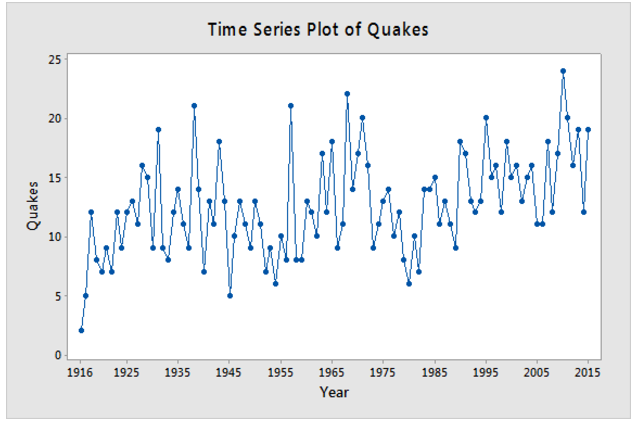
\includegraphics[width=130mm]{HinhTimeseries.png}
		\caption{Ví dụ về chuỗi thời gian động đất} 
		\label{HinhTimeseries.png}
	\end{center}
\end{figure}

Ngoài ra, còn có các định nghĩa về \textit{chuỗi thời gian đơn biến} (univariate time
series) và \textit{chuỗi thời gian đa biến} (multivariate time series). Chuỗi thời gian đơn biến
là một chuỗi thời gian chỉ chứa một quan sát được ghi nhận một cách tuần tự tại những
khoảng thời gian cách đều nhau. Chuỗi thời gian đa biến là chuỗi thời gian mà trong đó
tại một thời điểm ta có nhiều quan sát (biến) khác nhau.
\subsection{Chuỗi con}
Cho một chuỗi thời gian $T$ có chiều dài $n$, một \textit{chuỗi con} (Subsequence) $C$ của $T$ là một dãy có chiều dài $m$ ($1 \leq m \leq n$ ) có vị trí liền nhau trong chuỗi thời gian $T$.

Một chuỗi con $C$ của $T$ cũng có thể được xem là một chuỗi thời gian với chiều dài $m$. 
Một điều cần lưu ý là khái niệm “chuỗi con” khác với khái niệm “chuỗi tuần tự”. 
Nếu khái niệm “chuỗi tuần tự” cho phép các phần tử của chuỗi có thể không liên tục so với chuỗi ban đầu, thì khái niệm “chuỗi con $C$” của một chuỗi thời gian $T$ chỉ chấp nhận những phần tử liên tiếp nhau trong chuỗi thời gian $T$. 
Bên dưới là một ví dụ về chuỗi con của một chuỗi thời gian.

Cho chuỗi thời gian $T = (3, 5, 1, 12, 4, 7)$. 
Khi đó, $C_1 = (12, 4, 7)$ được gọi là một chuỗi con của chuỗi thời gian $T$. 
Tuy nhiên, $C_2 = (3, 1, 12, 4)$ không được xem là một chuỗi con của chuỗi thời gian $T$, vì $3$ và $1$ là các giá trị không liên tiếp nhau trong $T$.

Các công trình nghiên cứu thường áp dụng phương pháp \textit{cửa sổ trượt} (Sliding Windows) để lấy các chuỗi con trong một chuỗi thời gian để phục vụ cho bài toán nghiên cứu. 
Số lượng của các chuỗi con lấy được là bằng nhau và bằng độ dài của cửa sổ trượt. 
Hình \ref{chuoicon.png} minh họa chuỗi con được xác định bằng phương pháp cửa sổ trượt:

\begin{figure}
	\begin{center}
		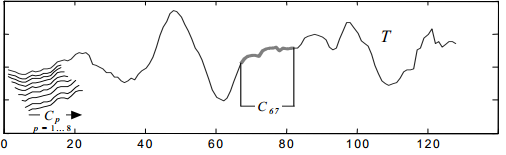
\includegraphics[width=120mm]{chuoicon.png}
		\caption{Ví dụ về chuỗi con và cửa sổ trượt [\ref{J. Lin}].}
		\label{chuoicon.png}
	\end{center}
\end{figure}
\subsection{Trùng khớp}
Cho một số thực dương $R$ (do người dùng định nghĩa) và một chuỗi thời gian $T$.
Biết rằng $T$ chứa một chuỗi con $C$ bắt đầu tại thời điểm $p$ và một chuỗi con $M$ bắt đầu tại $q$, nếu khoảng cách $D$ giữa 2 chuỗi nhỏ hơn hoặc bằng $R$, tức $D(C, M) \leq R$, thì $M$
là một \textit{chuỗi con trùng khớp} với $C$ và ngược lại.
\section{ĐỘ ĐO KHOẢNG CÁCH}
Có nhiều loại độ đo khoảng cách để hỗ trợ tính toán trong quá trình khai phá dữ liệu. 
Nhưng đối với quá trình phân lớp với tập dữ liệu chuỗi thời gian thì thường sử dụng 2 loại độ đo khoảng cách chủ yếu là độ đo khoảng cách Euclid và và độ đo khoảng cách xoắn thời gian động (Dynamic Time Warping -  DTW). 
Ở phần này chúng tôi tìm hiểu cách tính của 2 độ đo này trong dữ liệu chuỗi thời gian [\ref{E.keogh}].
\subsection{Khoảng cách Euclid}
Cho 2 chuỗi thời gian $Q = Q_1, Q_2,…., Q_n$ và $C = C_1, C_2, …, C_n$.
Khi đó khoảng cách Euclid giữa hai chuỗi thời gian $Q$ và $C$ được xác định bằng công thức sau:
\begin{align}
D\left( {Q, C} \right) = \sqrt[{}]{{\mathop \sum \limits_{i = 1}^n {{\left( {{q_i} - {c_i}} \right)}^2}}}
\end{align}

Độ đo khoảng cách Euclid có ưu điểm là dễ hiểu, dễ tính toán, dễ mở rộng cho nhiều bài toán khai phá dữ liệu chuỗi thời gian khác như gom cụm, phân lớp, nhận dạng mô típ, v.v.. 
Nhưng độ đo khoảng cách này có nhược điểm là nhạy cảm với nhiễu và thiếu sự mềm dẻo khi so trùng [\ref{Duong Tuan Anh}].
\subsection{Độ đo xoắn thời gian động (Dynamic Time Warping - DTW)}
Trên nhiều nghiên cứu đã chứng minh DTW là độ đo xoắn thời gian động tính toán khoảng cách giữa 2 mẫu dữ liệu chuỗi thời gian cho độ chính xác nhiều hơn so với khoảng cách Euclid. 
\subsubsection{Phương pháp tính khoảng cách DTW}
Cho 2 chuỗi thời gian $Q$ và $C$ có chiều dài lần lượt là $n$ và $m$ theo với $Q = Q_1, Q_2, …, Q_n$ và $C = C_1, C_2, …, C_m$ công thức DTW được tính như sau:
\begin{itemize}
\item Bước 1: Xây dựng một ma trận có kích thước $n*m$ với $n$ là số hàng của ma trận và $m$ là số cột của ma trận. 
Trong đó phần tử $(i^{th},j^{th})$ của ma trận chứa khoảng cách $d(q_i, c_j)$ giữa hai điểm $q_i, c_j$ trên 2 chuỗi dữ liệu $Q$ và $C$. Với $d(q_i, c_j) = (q_i - c_j)^2$.
\item Bước 2: Ma trận chứa khoảng cách $d(q_i, c_j)$ là ma trận xoắn. 
Một đường xoắn (warping path) là một tập các phần tử liên tục của ma trận định nghĩa một đường ánh xạ giữa $Q$ và $C$

$W = w_1, w_2, …, w_k$	 với $max(m, n) \le  K   \le m+ n -1$
\item Bước 3: Có rất nhiều đường xoắn thỏa mãn các điều kiện trên nhưng chúng ta chỉ quan tâm đến đường xoắn có chi phí tối thiểu.
Chi phí của một đường xoắn là tổng khoảng cách của các cặp điểm tương ứng với các ô nằm trên đường xoắn đó.
\begin{align}
DTW\left( {Q,C} \right) = \min \left\{ {\sqrt {\mathop \sum \limits_{k = 1}^K {W_k}} } \right.
\end{align}
Đường xoắn tối ưu này có thể tìm được bằng cách sử dụng phương pháp quy hoạch động (\textit{dynamic programming}). 
Công thức truy hồi cho khoảng cách tích lũy (\textit{cumulative distance})  được định nghĩa như sau:
\begin{equation}\label{eq.dtw}
\gamma(i, j) = d(d_i, c_j) + min
\begin{cases} 
      \gamma(i-1,j) \\
       \gamma(i,j-1) \\
       \gamma(i-1, j-1)
   \end{cases}
\end{equation}
Trong đó, khoảng cách tích lũy $\gamma(i, j)$ tại ô $(i, j)$ của ma trận được tính bằng khoảng cách của ô tương ứng cộng với giá trị nhỏ nhất của khoảng cách tích lũy của các ô liền kề trước ô đó.
Khoảng cách xoắn thời gian động của hai chuỗi thời gian $Q$ và $C$ là căn bậc hai của khoảng cách tích lũy tại ô có chỉ số là $(m,n)$.
\\
\\
Đối với việc tính toán DTW chúng ta có một số ràng buộc sau:
\begin{itemize}
\item Điều kiện biên: $w_1 = (1,1)$ và $w_k=(m, n)$ ràng buộc này yêu cầu đường xoắn phải bắt đầu và kết thúc ở hai góc đối diện của ma trận.
\item Tính liên tục: $w_k = (a,b)$ thì $w_{k-1} = (a', b')$ trong đó $a - a' \le 1$ và $b - b'  \le 1$. 
Ràng buộc này yêu cầu đường xoắn phải di chuyển giữa những ô liền kề (kể cả những ô liền kề theo đường chéo).
\item Tính đơn điệu tăng: $w_k = (a, b)$ thì $w_{k-1} = (a', b')$, với $a - a' \geq 0$ và $b - b' \geq 0$. 
Ràng buộc này yêu cầu các điểm trong đường xoắn $W$ phải có tính đơn điệu tăng theo thời gian.
\end{itemize}
Algorithm \ref{alg:DTW} trình bày mã giả giải thuật tính khoảng cách giữa hai chuỗi thời gian $Q$ có chiều dài $n$ và $C$ có chiều dài $m$.

\begin{algorithm}[h!]
  \caption{DTW
   \label{alg:DTW}}
    \textbf{Input:} $Q: Array[1.. n], C: Array[1 .. m]$\\
    \textbf{Output:} $DTW[n, m] $
  \begin{algorithmic}[1]
      \Let{$DTW$}{$empty Array[n, m]$}
      \For{from $i = $ to $n$}
          \For{from $j = 1$ to $m$}
              \State{// The distance $\gamma(i,j)$ is calculated using eq. \ref{eq.dtw}}
              \State{$DTW[i,j] = (Q[i]-C[j])^2 + min(DTW[i-1, j], DTW[i, j-1], DTW[i-1, j-1]$}
          \EndFor
      \EndFor
      \State \Return{$DTW[n, m]$}
  \end{algorithmic}
\end{algorithm}
Phương pháp DTW có ưu điểm là cho kết
quả chính xác hơn so với độ đo Euclid và cho phép nhận dạng mẫu có hình dạng giống nhau nhưng chiều dài hình dạng về thời gian có thể khác nhau. Phương pháp này có nhược điểm là thời gian chạy lâu, tuy nhiên cũng đã có những công trình nghiên cứu đề xuất các giải pháp tăng tốc độ tìm kiếm tương tự
dùng độ đo DTW.

Hình \ref{SosanhEu_DTW.png} mô tả sự khác biệt giữa độ đo Euclid và độ đo xoắn thời gian động.
\end{itemize}

\begin{figure}[h!]
	\begin{center}
		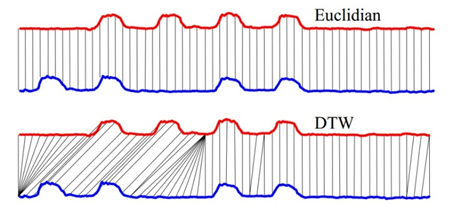
\includegraphics[width=110mm]{SosanhEu_DTW.png}
		\caption{Độ đo Euclid và độ đo xoắn thời gian động [\ref{E.keogh}] }
		\label{SosanhEu_DTW.png}
	\end{center}
\end{figure}

\begin{figure}[h!]
	\begin{center}
		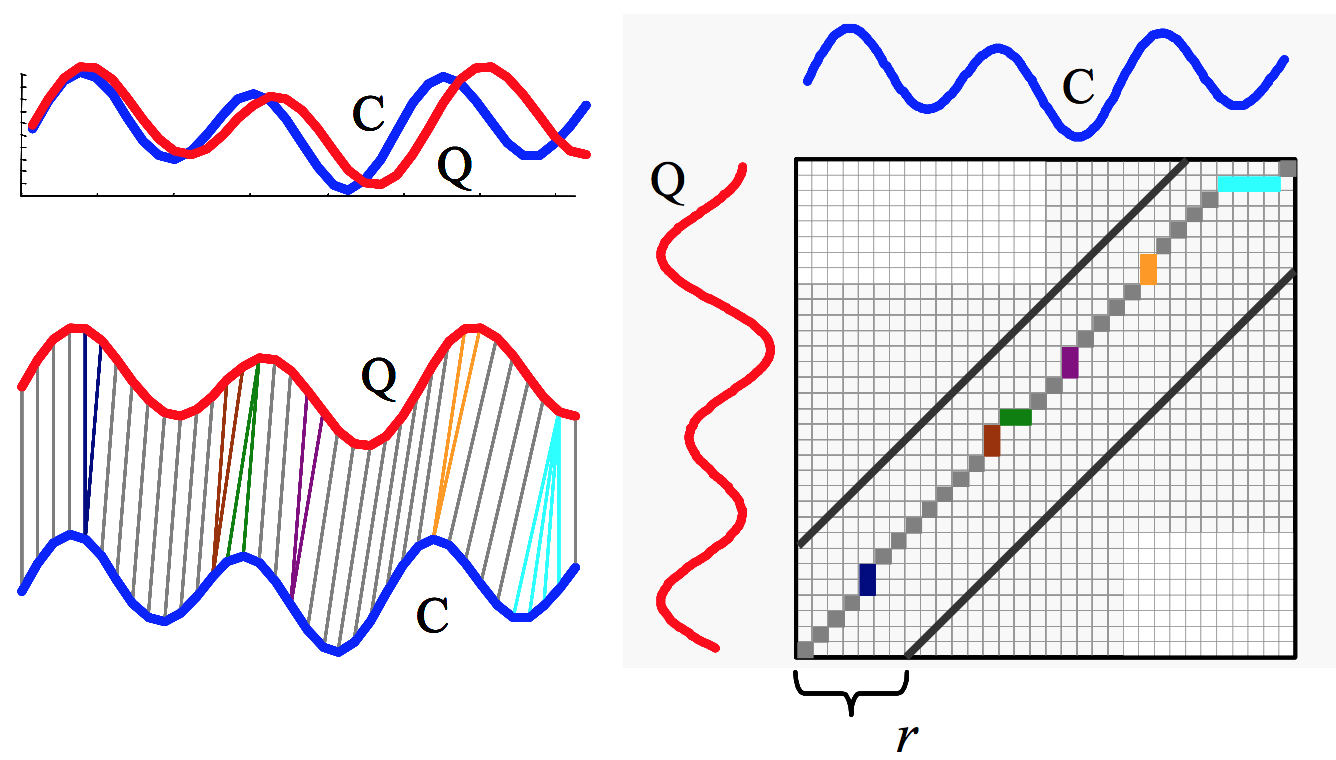
\includegraphics[width=110mm]{DTW.png}
		\caption{Ma trận xoắn thời gian động [\ref{Xi}] }
		\label{DTW.png}
	\end{center}
\end{figure}
Hình \ref{DTW.png} (bên trái) biểu diễn hai chuỗi thời gian $Q$ và $C$ tương tự nhau nhưng bị lệch giai đoạn (out of phase). Để sắp xếp lại hai chuỗi này ta xây dựng ma trận xoắn và tìm đường xoắn tối ưu (hình bên phải).
\subsubsection{Ví dụ tính khoảng cách DTW}
Giả sử có hai chuỗi thời gian $Q$ và $C$ như sau: \\
$Q=(1,3,4,9,8,2,1,5,7,3)$\\
$C=(1,6,2,3,0,9,4,3,6,3)$\\
Hai chuỗi thời gian $Q$ và $C$ được biểu diễn dưới dạng biểu đồ ở hình \ref{DTW_Example_Graph.png}
\floatplacement{figure}{H}
\begin{figure}[H]
	\begin{center}
		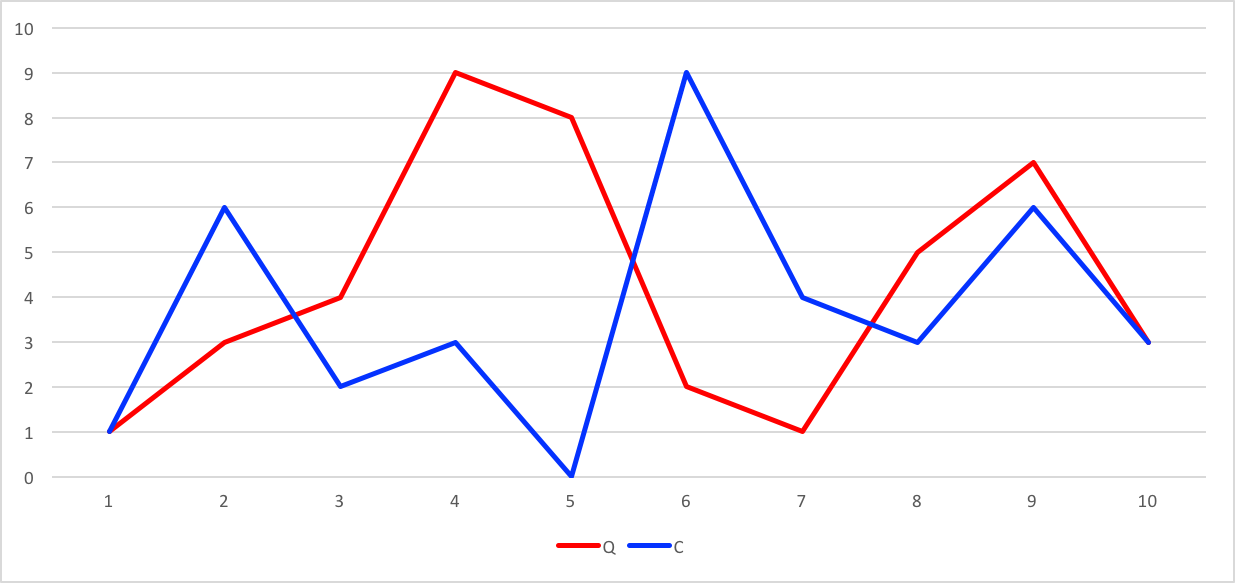
\includegraphics[width=110mm]{DTW_Example_Graph.png}
		\caption{Biểu đồ biểu diễn 2 chuỗi thời gian $Q$ và $C$}
		\label{DTW_Example_Graph.png}
	\end{center}
\end{figure}

Áp dụng Algorithm \ref{alg:DTW}, ta xây dựng ma trận xoắn lưu khoảng cách tích luỹ giữa các điểm dữ liệu tương ứng của hai chuỗi thời gian $Q$ và $C$.
Giá trị các phần tử $\gamma(i,j)$ trong ma trận được tính như sau:
\begin{equation}\label{eq.dtw}
\gamma(i, j) =
\begin{cases} 
      (Q_0 - C_0)^2 & \text{if $i = j = 0$} \\
      (Q_i - C_0)^2 + \gamma(i-1,0) & \text{if $i > 0, j = 0$} \\
       (Q_0 - C_j)^2 + \gamma(0, j-1) & \text{if $i = 0, j > 0$} \\
       (Q_i - C_j)^2 + min(\gamma(i, j-1), \gamma(i-1, j), \gamma(i-1, j-1)) & \text{if $i > 0, j > 0$} \\
   \end{cases}
\end{equation}

Khoảng cách giữa hai chuỗi thời gian $Q$ và $C$ là $\sqrt{\gamma(m,n)} = \sqrt{\gamma(10,10)} = \sqrt{15}$.
\begin{table}[!htb]
\centering
    \begin{tabular}{| c | c  c | c | c  | c | c | c | c | c | c | c | c | c | c | c |}
       \cline{1-1}\cline{4-13}
		3&&&33&23&19&16&19&23&18&18&18&\cellcolor{green}15\\
		\cline{1-1}\cline{4-13}
		7&&&31&20&18&16&19&17&18&19&\cellcolor{green}15&18\\
		\cline{1-1}\cline{4-13}
		5&&&25&19&13&12&16&15&15&15&\cellcolor{green}14&16\\
		\cline{1-1}\cline{4-13}
		1&&&21&18&10&11&11&19&14&\cellcolor{green}13&17&18\\ 
		\cline{1-1}\cline{4-13}
		2&&&21&13&9&10&12&16&\cellcolor{green}11&12&16&17\\
		\cline{1-1}\cline{4-13}
		8&&&20&9&13&16&19&\cellcolor{green}9&12&17&18&21\\ 
		\cline{1-1}\cline{4-13}
		9&&&13&7&11&11&14&\cellcolor{green}8&13&18&16&21\\
		\cline{1-1}\cline{4-13}
		4&&&5&4&5&5&\cellcolor{green}8&12&12&13&15&16\\
		\cline{1-1}\cline{4-13}
		3&&&2&\cellcolor{green}3&\cellcolor{green}4&\cellcolor{green}4&7&13&14&14&17&17\\
		\cline{1-1}\cline{4-13}
		1&&&\cellcolor{green}0&5&6&8&9&17&20&22&27&29\\ 
		\cline{1-1}\cline{4-13}
		\multicolumn{11}{l}{Q}\\
		\multicolumn{11}{l}{}\\
		\cline{4-13}
		\multicolumn{3}{r|}{C}&1&6&2&3&0&9&4&3&6&3\\
		\cline{4-13}
    \end{tabular}
    \caption{Ma trận khoảng cách giữa hai chuỗi thời gian $Q$ và $C$}\label{tab:dataset}
\end{table}

Dựa vào đường xoắn tìm được ta có mô hình biểu diễn sự tương quan giữa các điểm dữ liệu giữa hai chuỗi thời gian $Q$ và $C$ ở hình \ref{TW_Q-C.png}.
\begin{figure}[H]
	\begin{center}
		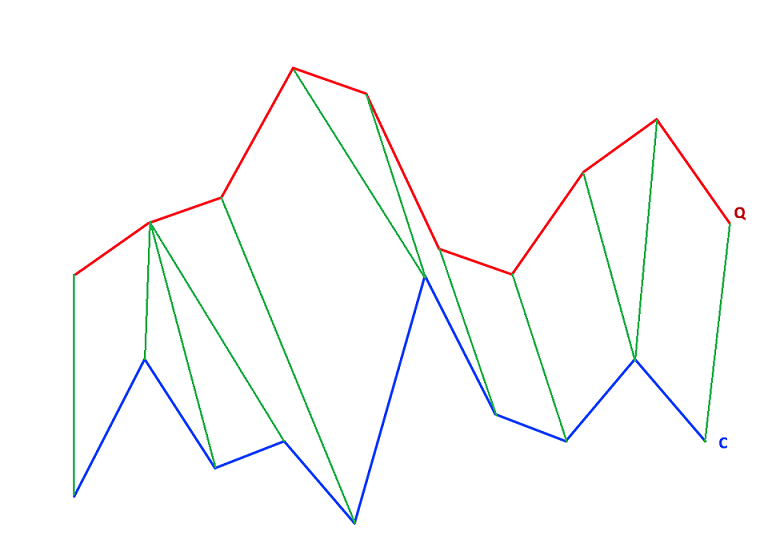
\includegraphics[width=120mm]{DTW_Q-C.png}
		\caption{Biểu đồ biểu diễn sự tương quan của 2 chuỗi thời gian $Q$ và $C$}
		\label{TW_Q-C.png}
	\end{center}
\end{figure}
\subsubsection{Các kỹ thuật tối ưu phương pháp DTW}
Việc tính độ đo xoắn thời gian động có chi phí lớn vì phải tìm đường xoắn đạt giá trị nhỏ nhất trong ma trận bằng phương pháp quy hoạch động. 
Độ phức tạp của giải thuật này là O(mn). 
Tuy nhiên, dựa trên ý tưởng cơ bản là giới hạn đường xoắn bằng cách thêm vào các giới hạn cục bộ trên tập hợp các bước sẽ xem xét, đã có hai ràng buộc về đường xoắn phổ biến là ràng buộc \textit{Sakoe - Chiba} và ràng buộc \textit{Hình bình hành Itakura}. 
Bằng cách định nghĩa một tập con của ma trận xoắn (\textit{wraping maxtrix}) chứa đường xoắn tối ưu. Tập con này được gọi là cửa sổ xoắn (\textit{wraping window}).
\begin{itemize}
	\item[*] \textit{\textbf {Ràng buộc dải Sakoe – Chiba}}
\end{itemize}
Kỹ thuật này được đề xuất bởi Sakoe và Chiba (1978) \ref{SakoeChiba}, ràng buộc này được mô tả như sau: \\
Gọi đường xoắn tối ưu là tập các ô trong ma trận của hai chuỗi thời gian:\\
$W = w_1, w_2, …, w_k$	 với $max(m, n) \le  K   \le m+ n -1$ \\
Trong đó $w_k = (i, j)_k$. Ràng buộc Sakoe-Chiba yêu cầu $|i - j| \le r$, trong đó $r$ là một số nguyên dương cho trước được gọi là cửa sổ xoắn. Minh hoạ ở hình \ref{SakoeChiba.png}
\begin{figure}[H]
	\begin{center}
		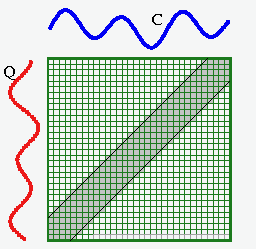
\includegraphics[width=60mm]{SakoeChiba.png}
		\caption{Ràng buộc Sakoe - Chiba}
		\label{SakoeChiba.png}
	\end{center}
\end{figure}
\begin{itemize}
	\item[*] \textit{\textbf {Ràng buộc hình bình hành Itakura (Itakura Paralelogram)}}
\end{itemize}
Kỹ thuật này được đề xuất bởi Itakura (1975). Ràng buộc này cũng định nghĩa đường xoắn nằm bên trong cửa sổ xoắn nhưng kích thước cửa sổ xoắn $r$ biến thiên theo thời gian, tạo nên hình bình hành. Hình \ref{Itakura.png} mô tả cửa sổ xoắn Itakura.

\begin{figure}[H]
	\begin{center}
		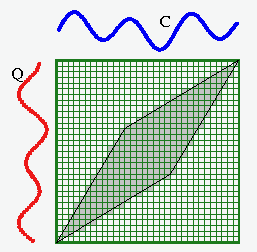
\includegraphics[width=60mm]{Itakura.png}
		\caption{Ràng buộc Hình bình hành Itakura}
		\label{Itakura.png}
	\end{center}
\end{figure}

Ràng buộc \textit{Sakoe - Chiba} và ràng buộc \textit{Hình bình hành Itakura} được xây dựng với mục đích chính là tăng tốc độ tính toán DTW thông qua việc giới hạn không gian tìm kiếm đường xoắn trong cửa sổ xoắn.
Điều này không có nghĩa là kích thước cửa sổ xoắn càng lớn thì đường xoắn tìm được càng tối ưu.
Trong một nghiên cứu của Keogh và cộng sự đã tiến hành thực nghiệm với việc kiễm tra độ chính xác phân lớp khi áp dụng kích thước cửa sổ xoắn tăng dần từ $0\%$ đến $100\%$.
Kết quả cho thấy cửa sổ xoắn có kích thước lớn hơn không cho ra độ chính xác tốt hơn.
Thông thường, độ chính xác phân lớp tốt nhất khi áp dụng kích thước cửa sổ xoắn khá nhỏ khoảng $4\%$ [\ref{E.keogh2}].
\section{CÁC PHƯƠNG PHÁP PHÂN LỚP DỮ LIỆU CHUỖI THỜI GIAN}
\subsection{Giải thuật phân lớp k-lân cận gần nhất (k-NN)}
k-NN là giải thuật được sử dụng rộng rãi trong nhiều bài toán phân lớp và dự báo.
Quy trình phân lớp của k-NN với một đối tượng $x_{new}$ được mô tả như sau:
\begin{itemize}
\item Tính khoảng cách giữa $x_{new}$ và tất cả các mẫu trong tập huấn luyện 
\item Chọn $k$ mẫu gần nhất với $x_{new}$ trong tập huấn luyện
\item Gán $x_{new}$ vào lớp có nhiều mẫu nhất trong số $k$ mẫu lân cận đó (hoặc $x_{new}$ nhận giá trị trung bình của $k$ mẫu)

Hình \ref{K-NN_Example.png} minh họa ví dụ phân lớp đối tượng mới vào lớp Dog hoặc Cat dựa vào k-lân cận gần nhất với trường hợp $k=1$
\end{itemize}
\begin{figure}[h!]
	\begin{center}
		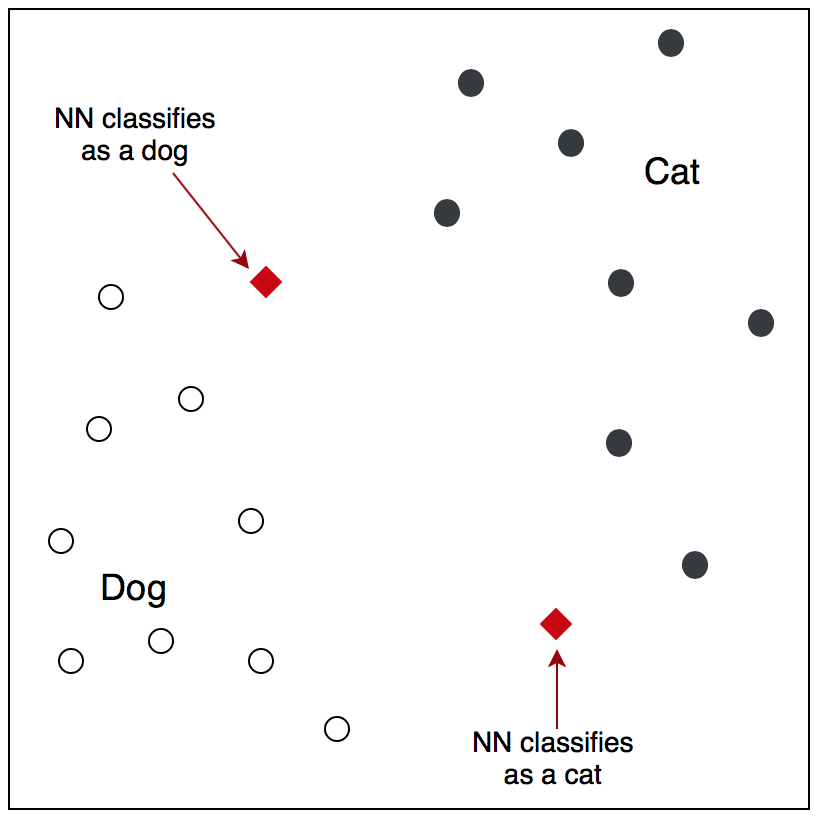
\includegraphics[width=90mm]{K-NN_Example.png}
		\caption{Phân lớp k-lân cận gần nhất}
		\label{K-NN_Example.png}
	\end{center}
\end{figure}
Ưu điểm:
\begin{itemize}
\item Dễ sử dụng và cài đặt
\item Xử lý tốt với dữ liệu nhiễu (do dựa trên khoảng cách để quyết định phân lớp)
\end{itemize}
Khuyết điểm:
\begin{itemize}
\item Cần lưu tất cả các mẫu để phân lớp
\item Cần nhiều thời gian để xác định lớp cho một mẫu mới (cần tính và so sánh khoảng cách đến tất cả các mẫu huấn luyện)
\item Phụ thuộc vào giá trị $k$ do người dùng lựa chọn. Nếu $k$ quá nhỏ, nhạy cảm với nhiễu. 
Nếu $k$ quá lớn thì vùng lân cận có thể chứa các điểm của lớp khác.
\item Cần chuyển đổi kiểu dữ liệu đối với thuộc tính rời rạc (categorical)
\end{itemize}
\subsection{Cây quyết định}
Cây quyết định là phương pháp phân lớp dưới dạng cấu trúc cây mà nó thực hiện kiểm tra phân tách tại mỗi nút nội và dự đoán phân lớp cho nút lá, nhánh từ một node nội là kết quả của một phép thử trên thuộc tính tương ứng. 
Đã có nhiều giải thuật khác nhau xây dựng cây quyết định áp dụng thành công trên nhiều lĩnh vực
[\ref{Decision tree}].
 Đặc điểm của các giải thuật này là:
\begin{itemize}
	\item Giải thuật tham lam (không có quay lui), chia để trị, đệ qui, từ trên xuống.
	\item Độ phức tạp với tập huấn luyện $D$ gồm $|D|$ phần	tử (đối tượng), mỗi phần tử gồm $n$ thuộc tính $O(n*|D|*log|D|)$.
	\begin{itemize}
		\item Mỗi thuộc tính ứng với mỗi cấp (level) của cây. 
		\item Cho mỗi cấp của cây, $|D|$ phần tử huấn luyện được
		duyệt qua.
	\end{itemize}
	\item Một bước quan trọng trong giải thuật là lựa chọn tiêu chí rẽ nhánh nghĩa là phân hoạch tập huấn luyện $D$ thành các phân hoạch con với các nhãn	phù hợp.
	\begin{itemize}
		\item Xếp hạng mỗi thuộc tính
		\item Thuộc tính được chọn để rẽ nhánh là thuộc tính có trị
		số điểm (score) lớn nhất
		\item Độ đo chọn thuộc tính phân tách (splitting attribute):
		độ lợi thông tin, chỉ số Gini
	\end{itemize}
\end{itemize}

Do dữ liệu chuỗi thời gian có những đặc điểm riêng (khối lượng dữ liệu lớn, giữa các điểm dữ liệu có mối tương quan với nhau và dữ liệu có thể có nhiễu) làm cho việc khai phá dữ liệu chuỗi thời gian trở nên khó khăn hơn.
Nhiều giải thuật phân lớp kinh điển làm việc tốt với dữ liệu thường nhưng không thể làm việc hiệu quả với dữ liệu chuỗi thời gian.
Qua các nghiên cứu đã cho thấy giải thuật phân lớp 1-NN sử dụng độ đo DTW phù hợp, có thể nói là tốt nhất với loại dữ liệu này (theo Wang và các cộng sự [\ref{DMKSWang}]).
\chapter{TỔNG QUAN CÁC CÔNG TRÌNH LIÊN QUAN}\label{Sec:Phan3}
Thu gọn dữ liệu chuỗi thời gian trở thành một bước tất yếu để tăng tốc quá trình phân lớp.
Nhiều công trình nghiên cứu đã cho ra đời những kỹ thuật thu gọn tập huấn luyện hiệu quả. 
Trong chương này chúng ta sẽ điểm qua một kỹ thuật thu gọn dữ liệu chuỗi thời gian tiên tiến hiện nay.
\section{KỸ THUẬT THU GỌN SỐ PHẦN TỬ TẬP HUẤN LUYỆN NAÏVE RANK}
Có nhiều giải thuật đề xuất cho vấn đề phân lớp với dữ liệu là chuỗi thời gian. 
Tuy nhiên, rõ ràng giải thuật một phần tử lân cận gần nhất (1-NN) với độ khoảng cách xoắn thời gian động (Dynamic Time Warping - DTW) là giải thuật đặc biệt khó có giải thuật nào đánh bại được [\ref{DMKSWang}]. 
Cách tiếp cận này có một điểm yếu, đòi hỏi tính toán nhiều trong thời gian thực. 
Có một cách khắc phục điểm yếu này là tăng tốc độ tính toán độ đo DTW. 
Xi và các cộng sự (2006) đã đưa ra kỹ thuật thu gọn số lượng (numerosity reduction) tập huấn luyện để tăng tốc độ giải thuật phân lớp 1-NN mà không làm mất tính chính xác phân lớp.

Kỹ thuật thu gọn số lượng tập huấn luyện có thể hiểu đơn giản là loại bỏ một số dữ liệu trong tập huấn luyện nhằm để cải thiện hiệu suất phân lớp. 
Nếu chúng ta cẩn thận lựa chọn đối tượng loại bỏ, chúng ta đặc biệt rút ngắn được thời gian phân lớp trong khi độ chính xác vẫn cao, trong một vài trường hợp tăng hiệu suất phân lớp một cách rất đáng kể.

Việc tăng tốc phân lớp dựa vào nền tảng kiến thức giải thuật k-NN và độ đo DTW đã trình bày ở Chương 2. 
Và quan trọng nhất là kỹ thuật thu gọn tập huấn luyện Naïve Rank (Naïve Rank Reduction) [\ref{Xi}].
Giải thuật Naïve Rank thu gọn tập huấn luyện gồm 2 bước là xếp hạng (ranking) và xác định ngưỡng (thresholding).
Đầu tiên giải thuật xếp hạng cho tất cả các đối tượng trong tập huấn luyện. 
Sau đó giải thuật xác định ngưỡng $n$ để quyết định có bao nhiêu đối tượng được giữ lại và $n$ đối tượng xếp hạng cao nhất được giữ lại để phân lớp.\\
Hạng của các đối tượng được xác định theo công thức \ref{eq.rank}: \\
\begin{equation}\label{eq.rank}
rank(x)=\sum_j
\begin{cases} 
      1 & \text{if class$(x)$ = class$(x_j)$} \\
       -2 & \text{otherwise}
   \end{cases}
\end{equation}

Với $x_j$ là đối tượng có $x$ là lân cận gần nhất.\\
Trường hợp 2 đối tượng có xếp hạng như nhau, thì sẽ dựa vào độ ưu tiên của chúng để phân biệt. Công thức tính độ ưu tiên của $x$ như sau:
\begin{equation}\label{eq.priority}
    priority(x) = \sum\limits_j {\frac{1}{{d{{(x, {x_j})}^2}}}}
\end{equation}
Với $x_j$ là đối tượng có $x$ là lân cận gần nhất và $d(x, x_j)$ là khoảng cách giữa $x$ và $x_j$. 
Nếu đối tượng ở cách xa lân cận gần nhất thì nó có thể là nhiễu hoặc không là đối tượng thuộc lớp thì nó được loại bỏ đi. 
Giữa 2 đối tượng có cùng xếp hạng nhưng đối tượng nào có độ ưu tiên thấp hơn sẽ bị loại bỏ đầu tiên.

Giải thuật xếp hạng có tính lặp. 
Giả sử tập huấn luyện có kích thước $N$, giải thuật sẽ chạy $N$ lần, tại mỗi lần lặp nó sẽ loại bỏ đối tượng có xếp hạng thấp và tiếp tục xếp hạng lại các đối tượng.

\begin{algorithm}[h!]
  \caption{Na{\"\i}ve Rank Reduction
   \label{alg:nrr}}
    \textbf{Input:} $T$\\
    \textbf{Output:} $S$
  \begin{algorithmic}[1]
      \State{Remove any duplicate instances from $T$}
      \State{leave -one-out 1-NN classification on $T$}
      \Let{$N$}{size of $T$}
      \Let{$S$}{$\emptyset$}
      \Let{$loop\_num$}{0}
      \While{$loop\_num$ < $N$}
          \For{each instance $x_i$ in $T$ - $S$}
              \State{rank$(x_i)$ is calculated using eq. \ref{eq.rank}}
          \EndFor
          \State{adjust the rank ties by priorities using eq. \ref{eq.priority}}
          \State{$worst\_index=arg_i(min(rank[x_i] \& min(priority[x_i])))$}
          \State{push($S, x_{worst\_index}$)} \textit{// discard instance with lowest rank}
          \Let{$loop\_num$}{$loop\_num + 1$}
      \EndWhile
      \State \Return{$S$}
  \end{algorithmic}
\end{algorithm}

Trong bước xác định ngưỡng, $n$ phần tử có hạng cao nhất được giữ lại trong  $S$ như là tập huấn luyện để làm đầu vào cho giải thuật phân lớp ($n$ là tham số đầu vào được xác định bởi người dùng).
Việc xác định ngưỡng có thể được dựa trên không gian hoặc thời gian tối đa mà người dùng có cho việc giải quyết bài toán.
Ví dụ, việc phân lớp côn trùng với tài nguyên hạn chế của các cảm biến (sensors), người dùng chỉ có tối đa 200k bộ nhớ để lưu toàn bộ tập huấn luyện (Wei \& Keogh, 2005).
Ngoài ra còn có một số cách xác định ngưỡng khác như \textit{"cho tập dữ liệu huấn luyện nhỏ nhất với một tỉ lệ lỗi mong đợi ít hơn 5\%"} hoặc \textit{"cho tập dữ liệu huấn luyện nhỏ nhất với tỉ lệ lỗi leave-one-out không khác với tỉ lệ lỗi trên toàn bộ tập dữ liệu quá 1\%"}.

Algorithm \ref{alg:nrr} trình bày mã giả của giải thuật thu gọn dữ liệu Naïve Rank, nhận vào tập huấn luyện $T$ và trả ra tập thu gọn $S$.
Giải thuật bắt đầu bằng việc loại bỏ các phần tử trùng lặp trong tập huấn luyện $T$ (dòng 1).
Sau đó tiến hành phân lớp sử dụng giải thuật 1-NN trên tập huấn luyện $T$ (dòng 2).
Mỗi phần tử trong tập huấn luyện được xác định thứ hạng sử dụng công thức \ref{eq.rank} (dòng 7-9).
Nếu thứ hạng các phần tử bị trùng nhau, thứ hạng sẽ được điều chỉnh bằng công thức \ref{eq.priority} (dòng 10).
Những phần tử có thứ hạng nhỏ nhất sẽ không được đưa vào tập kết quả $S$ (dòng 12).
Giải thuật dừng khi đã duyệt qua tất cả các phần tử trong tập huấn luyện $T$.
\section{PHƯƠNG PHÁP THU GỌN TẬP HUẤN LUYỆN INSIGHT}
Trong công trình này, Buza và các cộng sự [\ref{Buza}] đề xuất một phương pháp lựa chọn phần tử mới mà nó khai thác khái niệm của tính trung tâm (hubness), là một vài phần tử có xu hướng là lân cận gần nhất rất thường xuyên hơn những phần tử còn lại. 
Dựa trên tính trung tâm, họ đề xuất một khung sườn cho việc lựa chọn phần tử dựa trên điểm (score), nó được kết hợp với nguyên tắc tối ưu hóa độ bao phủ (coverage) của dữ liệu huấn luyện. 
Nghĩa là một chuỗi thời gian $x$ bao phủ một chuỗi thời gian $y$, nếu $y$ có thể được phân lớp đúng đắn dự trên $x$. 
Phương pháp này không chỉ cho phép hiểu tốt hơn bài toán lựa chọn phần tử mà còn giúp cho việc phân tích các đặc điểm của hướng tiếp cận từ quan điểm của việc tối đa hóa sự bao phủ. 
Với những lý do trên, hướng tiếp cận này được gọi là “Lựa chọn phần tử dựa trên sự bao phủ đồ thị và  tính trung tâm của chuỗi thời gian” (Instance Selection based on Graph-coverage and Hubness for Time-series), được viết tắt là INSIGHT.

INSIGHT được đánh giá thực nghiệm với 37 tập dữ liệu phân lớp chuỗi thời gian và được so sánh với FastAWARD, một phương pháp lựa chọn phần tử tiên tiến cho dữ liệu chỗi thời gian. 
INSIGHT được đánh giá là tốt hơn FastAWARD một cách đáng kể về cả độ chính xác phân lớp cũng như thời gian thực thi việc lựa chọn phần tử [\ref{Buza}].
\subsection{Hàm tính trọng số}

\subsubsection{Thuộc tính trung tâm}
Để xây dựng \textit{hàm trọng số} (score function) phục vụ việc lựa chọn phần tử đại diện cho phân lớp chuỗi thời gian bằng phương pháp lân cận gần nhất, ta phải kể đến phát hiện gần đây về thuộc tính trung tâm. 
Thuộc tính này chỉ ra rằng với dữ liệu cao chiều như hầu hết dữ liệu chuỗi thời gian, một vài đối tượng có xu hướng trở thành lân cận gần nhất thường xuyên hơn những đối tượng khác. 
Để diễn tả trung tâm một cách chính xác, cho một tập dữ liệu $\mathscr{D}$ chúng ta định nghĩa lần xuất hiện như là lân cận thứ $k$ ($k-occurrence$) của một phần tử $x \in \mathscr{D}$, ký hiệu $f^k_N(x)$ là số phần tử của $\mathscr{D}$ có $x$ ở giữa $k$ lân cận gần nhất. 
Với thuật ngữ \textit{trung tâm} (hubness) đề cập tới hiện tượng mà phân bố của $f^k_N(x)$  lệch đáng kể về bên phải. Độ lệch được ký hiệu: $\mathscr{S}_{f^k_N(x)}$

\begin{equation}
\mathscr{S}_{f^k_N(x)} = \frac{E[(f^k_N(x) - \upmu_{f^k_N(x)})^3]}{\upsigma^3_{f^k_N(x)}}
\end{equation}
Trong đó $\upmu_{f^k_N(x)}$ và $\upsigma_{f^k_N(x)}$ là trung vị và độ lệch chuẩn của $f^k_N(x)$.
Khi $\mathscr{S}_{f^k_N(x)}$ lớn hơn một thì phân bố tương ứng lệch về bên phải tạo thành đuôi dài.
Với dữ liệu có nhãn, trung tâm tốt và trung tâm xấu được phân biệt như sau: phần tử $y$ là một \textit{k-lân cận gần nhất} tốt (xấu) của phần tử $x$ nếu (i) $y$ là một trong $k$ lân cận gần nhất của $x$, và (ii) chúng có cùng (khác) nhãn.
Điều này cho phép định nghĩa \textit{k-occurence} tốt (xấu) của một chuỗi thời gian $x$, tương ứng là $f^k_G(x)$ (và $f^k_B(x)$) là số lượng những chuỗi thời gian khác mà có $x$ là một trong những \textit{k-lân cận gần nhất} tốt (xấu) của chúng.
\begin{figure}[h!]
	\begin{center}
		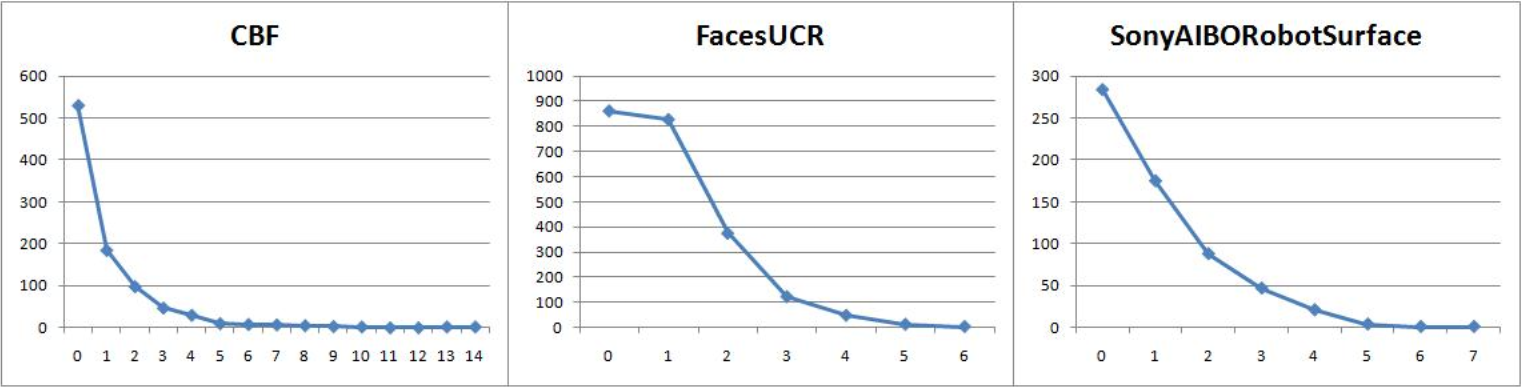
\includegraphics[width=160mm]{INSIGHT_Distribution.png}
		\caption{Biểu đồ phân bố của hàm $f^1_G(x)$ trên một số chuỗi thời gian. Trục hoành thể hiện giá trị $f^1_G(x)$, trục tung là số lượng phần tử có giá trị đó.}
		\label{INSIGHT_Distribution.png}
	\end{center}
\end{figure}

Đối với dữ liệu chuỗi thời gian, cả hai phân bố $f^k_G(x)$ và $f^k_B(x)$ đều thường lệch về bên phải. Ví dụ ở hình \ref{INSIGHT_Distribution.png} mô tả sự phân bố của hàm $f^1_G(x)$ trên một số chuỗi thời gian, biểu đồ phân bố tạo thành đuôi dài trong trường hợp trung tâm tốt (good hubs) xuất hiện.


Một chuỗi thời gian $x$ là một trung tâm tốt (xấu), nếu phân bố $f^k_G(x)$ ($f^k_B(x)$) rộng một cách đặt biệt với $x$. Đối với việc phân lớp chuỗi dữ liệu thời gian bằng phương pháp lân cận gần nhất thì việc biểu đồ phân bố lệch của các thể hiện tốt là rất quan trọng, bởi vì một số chuỗi thời gian có thể giúp phân lớp các chuỗi thời gian khác một cách đúng đắn. Vì thế, đây là bằng chứng quan trọng để ta nên đặc biệt chú ý vào các trung tâm tốt.
\subsubsection{Hàm tính trọng số dựa trên thuộc tính trung tâm}
Dựa vào \textbf{Good 1-occurence score} đã tìm thấy trước đó - giải thuật INSIGHT sử dụng trọng số của phần tử là 1-xuất hiện tốt. Công thức tính trọng số 1-xuất hiện tốt như sau:
\begin{equation}
f_G(x) = f^1_G(x)
\end{equation}

Trọng số tương đối (Relative Score) $f_R(x)$ của một chuỗi thời gian $x$ là phân số của 1-xuất hiện tốt và tổng xuất hiện cộng với một (để tránh trường hợp mẫu số là 0):
 \begin{equation}
f_R(x) = \frac{f^1_G(x)}{f^1_N(x)+1}
\end{equation}

\textbf{Trọng số Xi (Xi's score)}, dựa vào $f^k_G(x)$ và $f^k_B(x)$ cho phép chúng ta giải thích tiêu chí xếp hạng trong công trình của Xi bằng cách diễn tả chúng như là một dạng khác của trọng số tương đối.
\begin{equation}
f_{Xi}(x) = f^1_G(x) - 2f^1_B(x)
\end{equation}

Giải thuật INSIGHT lựa chọn những phần tử có thứ hạng cao (top-ranked). Tuy nhiên, trong khi xếp hạng các phần tử, chúng ta cần xem xét sự tương quan giữa chúng. Ví dụ, giải sử rằng phần tử có thứ hạng cao đầu tiên cho phép độ chính xác phân lớp 1-NN hầu như giống với phần tử có thứ hạng cao thứ hai. Vì thế sự đóng góp của phần tử có thứ hạng cao thứ 2 là không quan trọng trong tổng thể quá trình phân lớp. 
Giải thuật INSIGHT có 3 bước cơ bản được mô tả trong đoạn mã giả Algorithm \ref{alg:INSIGHT} sau:
\begin{itemize}
	\item Bước 1: Tính trọng số cho tất cả các phần tử $x$ trong $D$.
	\item Bước 2: Sắp xếp tất cả các chuỗi thời gian trong $D$ theo trọng số của chúng.
	\item Bước 3: Chọn $N$ chuỗi thời gian có thứ hạng cao đưa vào tập hợp kết quả.\end{itemize}
\begin{algorithm}
  \caption{INSIGHT
   \label{alg:INSIGHT}}
    \textbf{Require:} Time-series dataset $D$, Score Function $f$ , Number of selected instances $N$\\
    \textbf{Ensure:} Set of selected instances (time series) $D$
  \begin{algorithmic}[1]
          \State{Calculate score function $f(x)$ for all $x \in D$}
          \State{Sort all the time series in $D$ according to their scores $f(x)$}
          \State{Select the top-ranked $N$ time series and return the set containing them}
  \end{algorithmic}
\end{algorithm}

\section{PHÂN LỚP k-NN HIỆU QUẢ VỚI KỸ THUẬT GỌN DỮ LIỆU DỰA VÀO GOM CỤM PHI THAM SỐ}
\subsection{Thu gọn dựa vào gom cụm (RHC)}
RHC là giải thuật \textit{trích yếu đại diện} (prototype abstraction) phi tham số. 
Nó dựa vào ý tưởng đơn giản là áp dụng đệ quy vào giải thuật gom cụm k-means. 
Đặc biệt RHC xây dựng cụm cho đến khi chúng thuần nhất nghĩa là tất cả đối tượng chỉ thuộc về  cùng một lớp.
Ban đầu RHC xem toàn bộ tập huấn luyện là \textit{không thuần nhất} (non-homogeneous). 
Giải thuật bắt đầu tìm mean (centroid - trung tâm cụm) của mỗi lớp bằng cách tính toán trung bình các giá trị thuộc tính của các mẫu tương ứng của tập huấn luyện. 
Vì vậy một tập dữ liệu có $n$ lớp, giải thuật sẽ tính $n$ centroid. 
RHC thực thi giải thuật gom cụm k-means sử dụng $n$ centroid ban đầu và xây dựng các cụm. 
Đối với mỗi cụm thuần nhất centroid thuộc về \textit{tập ngưng tụ} (condensing set), còn cụm chưa thuần nhất tiếp tục thực hiện đệ quy lại thủ tục trên. 
Giải thuật ngừng khi tất cả các cụm đã thuần nhất. 
Khi kết thúc, tập ngưng tụ gồm tất cả các centroid của các cụm đã thuần nhất. 
Chú ý sử dụng mean của các lớp như là các centroid ban đầu cho giải thuật k-means, số lượng cụm sẽ được xác định tự động. 
Phần tử trung bình $m$ của một cụm hoặc lớp $C$ tính bằng cách lấy trung bình giá trị của $n$ thuộc tính của các phần tử $x_j, j = 1, 2,...,|C|$ trong $C$. Cụ thể, thuộc tính thứ $j$ của phần tử trung bình $m$ được xác định bởi công thức \ref{eq.mdj} sau đây:
\begin{equation}\label{eq.mdj}
m.{d_j} = \frac{1}{{\left| C \right|}}\sum\limits_{{x_i} \in C} {{x_i}.{d_j},j = 1,2,...,n} 
\end{equation}
Với
\begin{itemize}
\item $m$: một đối tượng nào đó trong cụm hoặc trong lớp tương ứng  $x_i, i= 1, 2. . .|C|$
\item $n$: là số thuộc tính.

\noindent Hình \ref{QuiTrinh_RHC} mô tả trực quan qui trình thực hiện giải thuật RHC.
\end{itemize}

\begin{figure}[h!]
	\begin{center}
		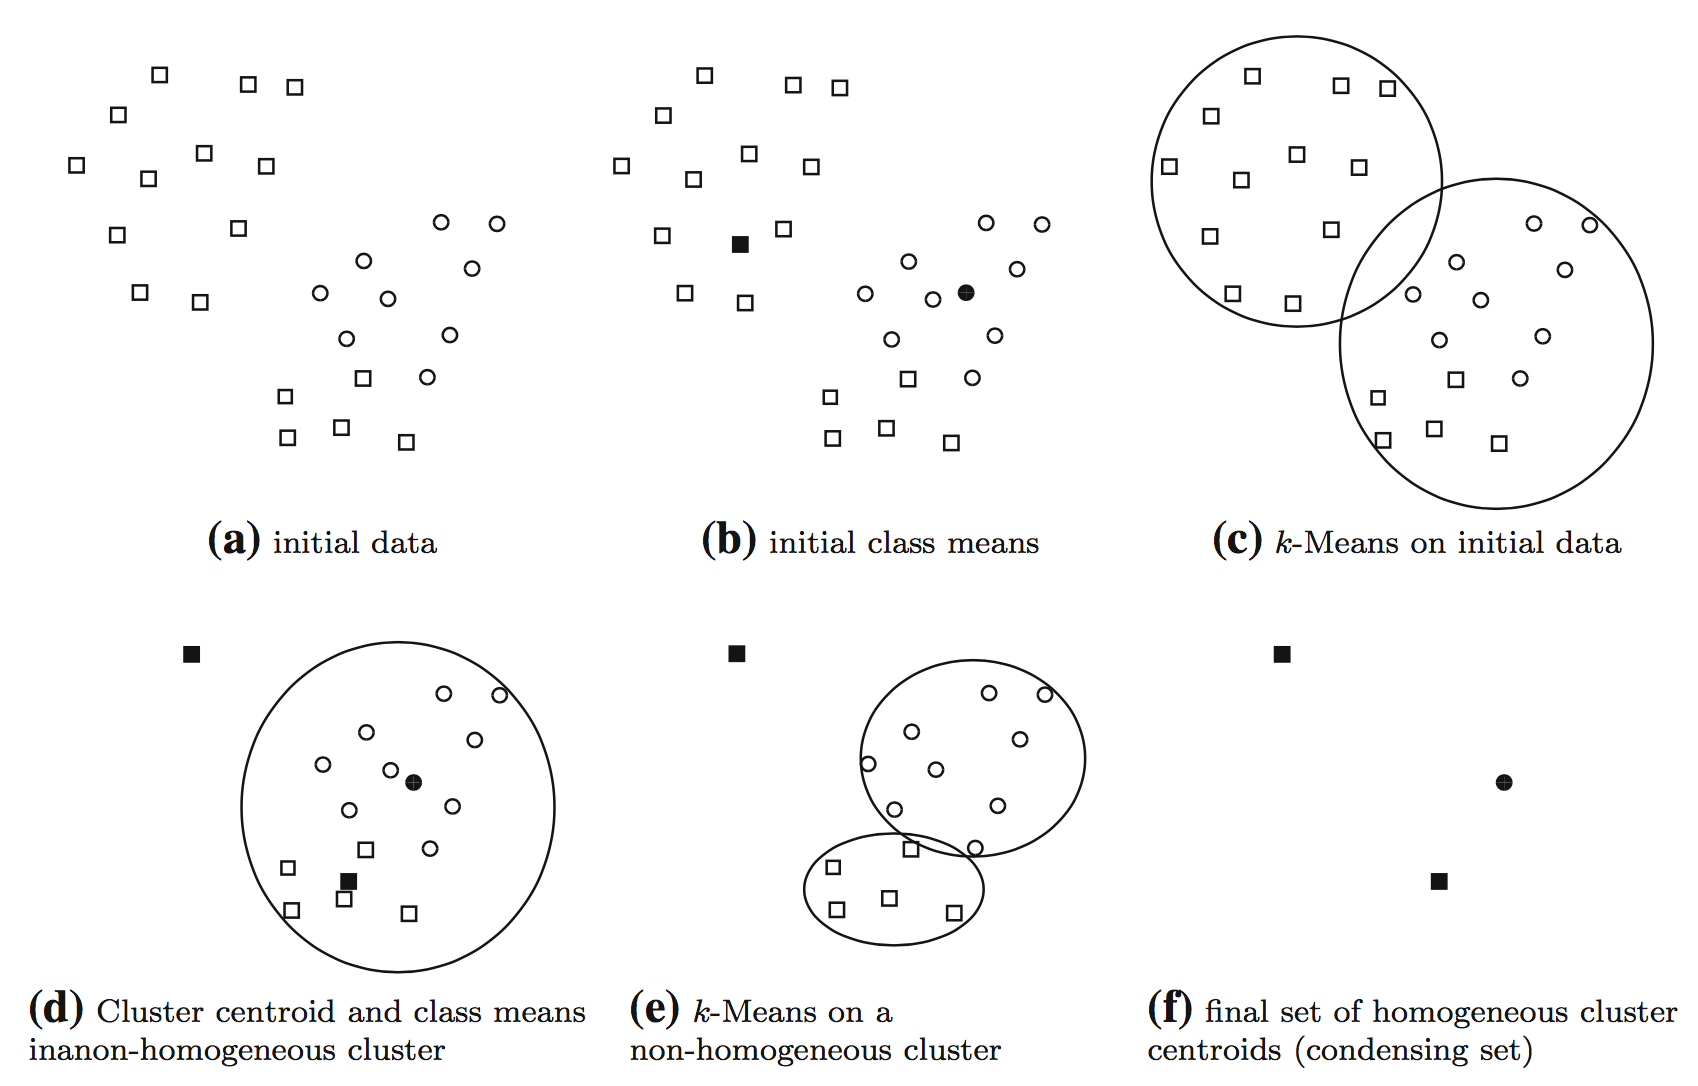
\includegraphics[width=140mm]{RHC.png}
		\caption{Quy trình thực hiện của giải thuật RHC [\ref{Stefanos Ougiaroglou}].}
		\label{QuiTrinh_RHC}
	\end{center}
\end{figure}

\begin{algorithm}[h!]
  \caption{RHC
   \label{alg:rhc}}
    \textbf{Input:} $TS$\\
    \textbf{Output:} $CS$
  \begin{algorithmic}[1]
    \Statex
      \\\textbf{\{Stage 1: Queue Initialization\}}
      \Let{$Queue$}{$\emptyset$}
      \\$Enqueue(Queue, TS)$
      \\\textbf{\{Stage 2: Construction of the condensing set\}}
      \Let{$CS$}{$\emptyset$}
      \Repeat
          \Let{$C$}{Dequeue($Queue$)}
          \If{$C$ is homogenious }
          \Let{$r$}{mean of $C$}
          \Let{$CS$}{$CS \cup \{r\}$}
      \Else
          \Let{$M$}{$\emptyset$} \{M is the set of class means\}
          \For{each class $L$ in $C$}
              \Let{$m_L$}{mean of $L$}
              \Let{$M$}{$M \cup \{m_L\}$}
          \EndFor
          \Let{$NewClusters$}{K-Means($C,M$)}
          \For{each cluster $NC \in NewClusters$}
              \State {$Enqueue(Queue, NC)$}
          \EndFor
      \EndIf
      \Until{IsEmpty($Queue$)}
      \State \Return{$CS$}
  \end{algorithmic}
\end{algorithm}

Algorithm \ref{alg:rhc} trình bày mã giả của giải thuật RHC.
Nó tận dụng cấu trúc dữ liệu hàng đợi, $Queue$ để lưu các cụm.
Đầu tiên, giải thuật RHC xem toàn bộ tập huấn luyện $TS$ như là một cụm chưa được xử lý. Do đó nó được đặt vào hàng đợi $Queue$ (dòng 3).
Ở mỗi bước lặp, giải thuật RHC xét phần tử $C$ đầu hàng đợi $Queue$ (dòng 7).
Sau đó nó kiểm tra xem $C$ có phải là cụm thuần nhất hay không.
Nếu $C$ là cụm thuần nhất (dòng 8) thì phần tử trung bình $r$ của $C$ được thêm vào tập ngưng tụ (dòng 10).
Ngược lại nếu $C$ là tập không thuần nhất thì giải thuật RHC tính các trung bình lớp $M$: một trung bình lớp cho mỗi lớp trong $C$ (dòng 13-16).
Sau đó, giải thuật RHC sử dụng giải thuật gom cụm k-means với tham số đầu vào là $C$ và $M$, tạo ra một tập hợp các cụm mới (dòng 17) và thêm vào hàng đợi $Queue$ (dòng 18-20).
Giải thuật dừng lại khi không còn phần tử nào trong hàng đợi $Queue$ (dòng 22) hay nói cách khác là khi tất cả các cụm đều thuần nhất.
\subsection{RHC động (dRHC)}
Giống với hầu hết các kỹ thuật thu gọn dữ liệu, RHC là kỹ thuật dựa vào bộ nhớ, nghĩa là toàn bộ tập dữ liệu thuộc về bộ nhớ. 
RHC không thể quản lý hết tập dữ liệu vì không thể lưu hết dữ liệu vào bộ nhớ chính. 
Do vậy, nó không thể thực thi trên thiết bị bị giới hạn về bộ nhớ và cũng không thể chuyển dữ liệu qua các máy khác xử lý thông qua mạng máy tính. 
Vì đây là thủ tục tốn nhiều thời gian và chi phí. 
Thêm vào đó, RHC không thể xử lý khi có những mẫu dữ liệu mới thêm vào. 
Giả sử RHC được thực thi trên tập dữ liệu $D$ và xây dựng tập ngưng tụ. 
Sau đó giả sử một tập dữ liệu mới $S$ được đưa thêm vào xem xét. 
Để xây dựng cập nhật lại tập ngưng tụ, RHC phải thực thi lại từ đầu trên tập 
$D \cup S$. 
Thủ tục phải thực hiện lặp lại  bất cứ khi nào có tập dữ liệu mới thêm vào, lúc này nhu cầu lưu trữ và chi phí tính toán cao.

Giải thuật dRHC là phiên bản động của RHC, nó kế thừa lại tất cả ưu điểm của RHC. 
Nhưng nó khắc phục được điểm yếu của RHC, nếu tập dữ liệu không phù hợp với bộ nhớ chính, nó sẽ chia tập dữ liệu thành các “phân đoạn dữ liệu” (data segments) để thích hợp với kích thước bộ nhớ chính. 
Ngoài ra đối với môi trường động khi dữ liệu đến liên tục, nó xem dữ liệu này như các “phân đoạn dữ liệu”. 
Trong trường hợp này, khái niệm phân đoạn dữ liệu được thực hiện sử dụng bộ đệm (buffer), nơi tập dữ liệu mới được lưu trữ. 
Khi bộ đệm đầy, giải thuật dRHC bắt đầu thực thi trên chúng. 
Sau đó tập dữ liệu được lưu trữ trong bộ đệm bị xóa đi và bộ đệm sẵn sàng nhận tập dữ liệu mới. 
dRHC thực hiện 2 giai đoạn: 
(1) xây dựng tập ngưng tụ ban đầu (CS-consending set), 
(2) cập nhật tập ngưng tụ mỗi lần một phân đoạn dữ liệu đến. 
Mọi thủ tục đều tương tự RHC, điểm khác biệt duy nhất giữa RHC và dRHC là mỗi lần sinh ra phần tử đại diện (prototype) lưu trữ giá trị trọng số như một thuộc tính bổ sung. 
Giá trị này là số lượng tập huấn luyện mà được gom lại với nhau và được đại diện bởi prototype đặc biệt trong tập ngưng tụ. 
Cập nhật tập ngưng tụ $CS$ chỉ dựa vào khái niệm cụm thuần nhất và các trọng số dữ liệu.
Công thức \ref{eq.drhc.weight} dưới đây là công thức tìm trung tâm cụm của dRHC:
\begin{equation}\label{eq.drhc.weight}
{m_C}.{d_j} = \frac{{\sum\limits_{{x_i} \in C} {{x_i}.{d_j} \times {x_i}.weight} }}{{\sum\limits_{{x_i} \in C} {{x_i}.weight} }}
\end{equation}
\begin{itemize}
\item $m$: đối tượng nào đó trong cụm hoặc trong lớp tương ứng  $x_i, i= 1, 2. . .|C|$
\item $d_j$ là mỗi vector thuộc tính của $m_C$, với $j = 1, 2,... n$

\end{itemize}
Quy trình thực hiện giải thuật dRHC được minh hoạ trực quan thông qua hình vẽ \ref{dRHC.png}.
\begin{figure}[h!]
	\begin{center}
		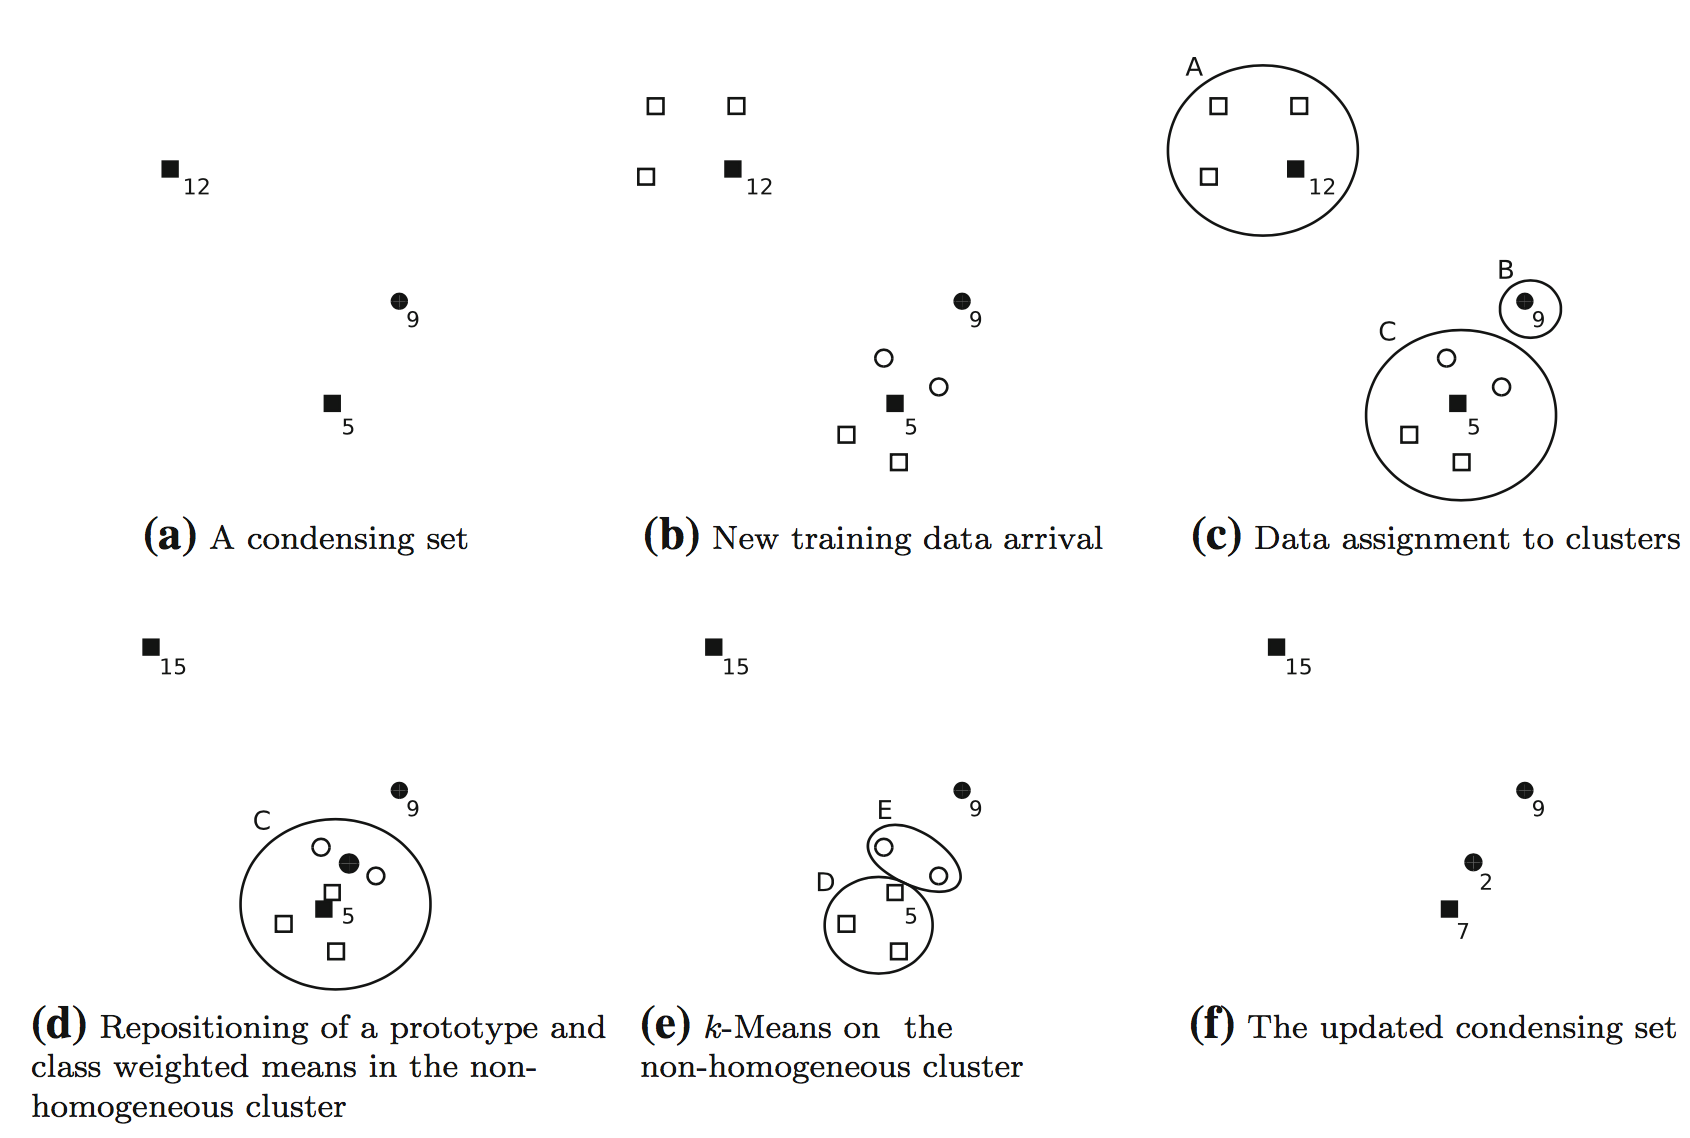
\includegraphics[width=145mm]{dRHC.png}
		\caption{Quy trình thực hiện giải thuật dRHC [\ref{Stefanos Ougiaroglou}]}
		\label{dRHC.png}
	\end{center}
\end{figure}

Algorithm \ref{alg:drhc} trình bày mã giả của giai đoạn cập nhật tập ngưng tụ $CS$ của giải thuật dRHC.
Nó nhận vào tập ngưng tụ sẵn có $oldCS$ cùng với một phân đoạn dữ liệu mới $dataSeg$ và trả ra tập ngưng tụ đã được cập nhật $newCS$.
Giải thuật bắt đầu bằng việc xây dựng hàng đợi $Queue$ để chứa những cụm chưa được xử lý.
Đầu tiên, nó khởi tạo một số lượng các cụm $CList$ bằng với số lượng phần tử trong tập ngưng tụ sẵn có $oldCS$ (dòng 3-6).
Tiếp theo, mỗi phần tử trong phân đoạn dữ liệu $dataSeg$ sẽ được gán trọng số là 1 và thêm vào một trong các cụm này (dòng 7-11).
Tất cả các cụm trong $CList$ được đặt vào hàng đợi $Queue$ (dòng 12-14).
Giải thuật dRHC tạo ra tập ngưng tụ mới $newCS$ bằng cách tương tự như $RHC$ nhưng có xem xét tới giá trị trọng số.
Đối với cụm thuần nhất thì phần tử đại diện được lưu trong $newCS$ là phần tử trung tâm cụm (dòng 19-22).
Đối với cụm không thuần nhất $C$, mỗi trung bình lớp được được đánh trọng số là tổng trọng số của các phần tử của lớp (dòng 24-29).
Những phần tử trung bình lớp này đóng vai trò là những phần tử trung bình khởi đầu cho giải thuật k-means (dòng 30). 
Giải thuật dRHC sử dụng giải thuật gom cụm k-means có quan tâm tới trọng số khi xác định trung tâm cụm.
Cho một cụm $C$, mỗi thuộc tính $d_j, j=1,2,..,n$ của trung tâm cụm $m_c$ (dòng 20, 26) được tính dựa vào công thức (\ref{eq.drhc.weight}). 
\begin{algorithm}
  \caption{dRHC: CS update phase 
   \label{alg:drhc}}
    \textbf{Input:} $oldCS, dataSeg$\\
    \textbf{Output:} $newCS$
  \begin{algorithmic}[1]
    \Statex
      \\\textbf{\{Stage 1: Queue Initialization\}}
      \Let{$Queue$}{$\emptyset$}
      \Let{$C List$}{$\emptyset$} \{empty list of clusters\}
      \For {each prototype $m \in oldCS$}
          \State {add new cluster $C = \{m\}$ in $C List$}
      \EndFor
      \For {each item $x \in dataSeg$}
          \State{$x.weight = 1$}
          \State{Find $C_x \in C List$ with the nearest to $x$ mean}
          \Let{$C_x$}{$C_x \cup \{x\}$} \{do not recompute mean of $C_x$\}
      \EndFor
      \For {each cluster $C$ in $C List$}
          \State{Enqueue($Queue, C$)}
      \EndFor
      \\\textbf{\{Stage 2: Construction of newCS\}}
      \Let{$newCS$}{$\emptyset$}
      \Repeat
          \Let{$C$}{Dequeue($Queue$)}
          \If{$C$ is homogenious }
          \Let{$m$}{weighted mean of $C$}
          \Let{$m.weight$}{$\sum\limits_{{x_i} \in C} {{x_i}.weight} $}
          \Let{$newCS$}{$newCS \cup \{m\}$}
      \Else
          \Let{$M$}{$\emptyset$} \{M is the set of weighted class means\}
          \For{each class $L$ in $C$}
              \Let{$m_L$}{mean of $L$}
              \Let{$m_L.weight$}{$\sum\limits_{{x_i} \in L} {{x_i}.weight} $}
              \Let{$M$}{$M \cup \{m_L\}$}
         
          \EndFor
          \Let{$NewClusters$}{K-Means($C,M$)}
          \For{each cluster $NC \in NewClusters$}
              \State {$Enqueue(Queue, NC)$}
          \EndFor
      \EndIf
      \Until{IsEmpty($Queue$)}
      \State \Return{$newCS$}
  \end{algorithmic}
\end{algorithm}
\newpage
\section{ÁP DỤNG CÁC GIẢI THUẬT LỰA CHỌN ĐẠI DIỆN VÀ TRÍCH YẾU ĐẠI DIỆN ĐỂ PHÂN LỚP DỮ LIỆU CHUỖI THỜI GIAN HIỆU QUẢ}
Các kỹ thuật thu gọn dữ liệu (Data Reduction Techniques - DRTs) trong phần này đều dựa trên ý tưởng đơn giản là: những phần tử không đại diện cho ranh giới quyết định giữa các lớp là những phần tử vô ích cho quá trình phân lớp. Do đó, chúng có thể bị loại bỏ. Giải thuật phân lớp k-NN đạt được độ chính xác gần như nhau khi thực hiện phân lớp trên tập huấn luyện và tập ngưng tụ. Việc duyệt qua tập ngưng tụ hiệu quả hơn duyệt qua tập huấn luyện. Do đó, các kỹ thuật thu gọn dữ liệu cố gắng lựa chọn hoặc tạo ra một số lượng vừa đủ các các phần tử nằm trong vùng dữ liệu gần với ranh giới quyết định. Các kỹ thuật thu gọn dữ liệu được trình bày trong phần này là phi tham số. Chúng xác định kích thước của tập ngưng tụ một cách tự động dựa trên mức độ nhiễu (noise) và số lượng lớp trong dữ liệu ban đầu (càng nhiều lớp, các nhiều ranh giới, do đó, càng nhiều phần tử được chọn hoặc tạo ra).
\subsection{Các giải thuật lựa chọn đại diện (Prototype Selection Algorithms)}
\subsubsection{Giải thuật CNN-rule}
CNN-rule [\ref{Hart}] là giải thuật lựa chọn đại diện (PS) ra đời sớm nhất và nổi tiếng nhất. 
Nó sử dụng hai tập hợp $CS$ và $TS$. 
Đầu tiên, một phần tử trong tập huấn luyện được đưa vào $CS$, những phần tử còn lại trong tập huấn luyện để trong tập $TS$.
Sau đó, CNN-rule cố gắng phân lớp tập $TS$ bằng cách sử dụng giải thuật phân lớp 1-NN trên nội dung của tập $CS$.
Khi một phần tử bị phân loại sai, nó được xem xét như nằm trong vùng dữ liệu gần ranh giới quyết định.
Vì thế nó được chuyển từ tập $TS$ sang tập $CS$.
Giải thuật ngừng lại khi không còn có sự chuyển dữ liệu từ tập $TS$ sang tập $CS$.

Mã giả của giải thuật CNN-rule được trình bày trong Algorithm \ref{alg:cnn-rule}: nó bắt đầu với một tập huấn luyện $TS$ và trả về một tập ngưng tụ $CS$. Ban đầu, $CS$ chỉ chứa một phần tử huấn luyện (dòng 1, 2). 
Sau đó, với mỗi phần tử huấn luyện $x \in TS$ (dòng 5), giải thuật truy xuất và kiểm tra nhãn lớp của lân cận gần nhất của nó (dòng 6).
Nếu nhãn lớp của $x$ khác với nhãn lớp của lân cận gần nhất của nó (dòng 7), $x$ sẽ được chuyển vào tập $CS$ (dòng 8, 9).
Quá trình này được lặp (dòng 4,10,13) đến khi không còn phần tử nào trong tập $TS$ được chuyển vào tập $CS$.
\begin{algorithm}[h!]
  \caption{CNN-rule
   \label{alg:cnn-rule}}
    \textbf{Input:} $TS$\\
    \textbf{Output:} $CS$
  \begin{algorithmic}[1]
      \Let{$CS$}{$\emptyset$}
      \\{pick an item of $TS$ and move it to $CS$}
      \Repeat
          \Let{$stop$}{$TRUE$}
          \For{each $x \in TS$}
              \Let{$NN$}{Nearest Neighbour of $x$ in $CS$}
              \If{$NN_{class} \neq x_{class}$}
              \Let{$CS$}{$CS \cup \{x\}$}
              \Let{$TS$}{$TS-\{x\}$}
              \Let{$stop$}{$FALSE$}
              \EndIf
          \EndFor
       \Until{$stop==TRUE$}
       \\{discard $TS$}
       \State \Return{$CS$}
  \end{algorithmic}
\end{algorithm}

Giải thuật CNN-rule dựa trên ý tưởng đơn giản là: những phần tử mà được phân lớp một cách đúng đắn bởi giải thuật 1-NN thì được xem là đang ở trung tâm lớp của vùng dữ liệu và vì thế chúng sẽ được bỏ qua. 
Nói cách khác, những phần tử mà phân lớp sai (misclassified) thì được xem là nằm gần đường biên lớp của vùng dữ liệu và vì thế chúng được đưa vào tập ngưng tụ. 
Điểm yếu của giải thuật CNN-rule là việc tạo ra kết quả tập ngưng tụ phụ thuộc vào thứ tự các phần tử trong tập huấn luyện.
Điều này có nghĩa là có thể có nhiều tập ngưng tụ khác nhau được tạo ra bởi cùng một tập huấn luyện với các thứ tự phần tử khác nhau.
\subsubsection{Giải thuật IB2}
Giải thuật IB2 thuộc họ các giải thuật học dựa trên phần tử (Instance-Based Learning - IBL) nổi tiếng và dựa  trên giải thuật CNN-rule.
Algorithm \ref{alg:ib2} trình bày mã giả của giải thuật IB2.
Mỗi phần tử trong tập huấn luyện $x \in TS$ được phân lớp bằng giải thuật phân lớp 1-NN dựa trên tập ngưng tụ $CS$ tại thời điểm hiện tại (dòng 4).
Nếu $x$ được phân lớp đúng, nó sẽ bị loại bỏ (dòng 8).
Ngược lại, $x$ sẽ được chuyển vào tập ngưng tụ $CS$ (dòng 6).
Trái với giải thuật CNN-rule, giải thuật IB2 không đảm bảo mọi phần tử bị loại bỏ đều có thể được phân lớp một cách đúng đắn dựa vào tập ngưng tụ.
Tuy nhiên, IB2 là giải thuật duyệt một lần (one-pass algorithm) nên nó rất nhanh, chi phí tính toán tiền xử lý thấp.
Thêm vào đó, giải thuật IB2 xây dựng tập ngưng tụ một cách gia tăng nên rất thích hợp cho môi trường động, phát trực tuyến nơi mà các phần tử huấn luyện mới được thêm vào một cách liên tục.
Ngoài ra, giải thuật IB2 còn khác với giải thuật CNN-rule và các kỹ thuật thu gọn dữ liệu khác ở chỗ giải thuật IB2 không đòi hỏi toàn bộ tập huấn luyện phải được lưu trong bộ nhớ.
Vì thế, giải thuật IB2 có thể được ứng dụng trên các thiết bị có bộ nhớ hạn chế không thể chứa toàn bộ tập huấn luyện.
Và cũng giống như giải thuật CNN-rule, IB2 cũng là giải thuật phụ thuộc vào thứ tự của tập huấn luyện.

\begin{algorithm}[h!]
  \caption{IB2
   \label{alg:ib2}}
    \textbf{Input:} $TS$\\
    \textbf{Output:} $CS$
  \begin{algorithmic}[1]
      \Let{$CS$}{$\emptyset$}
      \\{an item is chosen at random to migrate from $TS$ to $CS$}
       \For{each $x \in TS$}
           \Let{$NN$}{Nearest Neighbour of $x$ in $CS$}
           \If{$NN_{class} \neq x_{class}$}
             \Let{$CS$}{$CS \cup \{x\}$}
            \EndIf
            \Let{$TS$}{$TS-\{x\}$}
          \EndFor
       \State \Return{$CS$}
  \end{algorithmic}
\end{algorithm}
\subsection{Các giải thuật trích yếu đại diện (Prototype Abstraction Algorithms)}
\subsubsection{Giải thuật trích yếu IB2 (AIB2)}
Giải thuật AIB2 là phiên bản trích yếu đại diện (PA) của giải thuật IB2.
Vì thế, nó kế thừa tất cả các đặc điểm của giải thuật IB2.
Ý tưởng của giải thuật AIB2 rất đơn giản: những phần tử đại điện phải nằm ở trung tâm của vùng dữ liệu mà nó đại diện.
Do đó, những phần tử được phân lớp đúng không bị loại bỏ. 
Những phần tử này góp phần tạo ra tập ngưng tụ bằng cách định vị lại những đại diện gần nhất của chúng bằng cách áp dụng khái niệm trọng số.
Mỗi đại diện được đặc trưng bởi một trọng số biểu thị số lượng phần tử mà nó đại diện.
\begin{algorithm}[h!]
  \caption{AIB2
   \label{alg:aib2}}
    \textbf{Input:} $TS$\\
    \textbf{Output:} $CS$
  \begin{algorithmic}[1]
      \Let{$CS$}{$\emptyset$}
      \\{move a random item $y$ from $TS$ to $CS$}
      \Let{$y_{weight}$}{1}
       \For{each $x \in TS$}
           \Let{$NN$}{Nearest Neighbour of $x$ in $CS$}
           \If{$NN_{class} \neq x_{class}$}
             \Let{$x_{weight}$}{1}
             \Let{$CS$}{$CS \cup \{x\}$}
           \Else
             \For{each attribute $attr(i)$}
             \Let{$NN_{attr(i)}$}{$\frac{NN_{attr(i)} \times NN_{weight}+x_{attr(i)}}{NN_{weight}+1}$}
             \EndFor
             \Let{$NN_{weight}$}{$NN_{weight} + 1$}
           \EndIf
           \Let{$TS$}{$TS-\{x\}$}
          \EndFor
       \State \Return{$CS$}
  \end{algorithmic}
\end{algorithm}

Algorithm \ref{alg:aib2} hiện thực giải thuật AIB2 bằng mã giả.
Đầu tiên, tập ngưng tụ $CS$ chỉ có một phần tử duy nhất với trọng số khởi tạo là 1 (dòng 1-3).
Với mỗi phần tử huấn luyện $x$, giải thuật AIB2 truy xuất đại diện gần nhất của nó $NN$ từ tập ngưng tụ hiện hành (dòng 6-8).
Những thuộc tính của $NN$ được cập nhật bằng cách tính đến trọng số hiện tại của nó và các thuộc tính của $x$.
Kết quả là $NN$ tiến về phía $x$ (dòng 10-12). 
Cuối cùng, trọng số của $NN$ được tăng lên một đơn vị (dòng 13) và $x$ bị loại bỏ (dòng 15).

Giải thuật AIB2 hướng tới mục đích nâng cao hiệu của giải thuật IB2 bằng cách xây dựng tập ngưng tụ với những phần tử đại diện tốt hơn giải thuật IB2.
Mỗi đại diện nằm gần với trung tâm của vùng dữ liệu mà nó đại diện.
Do vậy, AIB2 có thể đạt được độ chính xác phân lớp cao hơn.
Hơn thế nữa, những đại diện được định vị lại góp phần làm giảm số lượng phần tử trong tập ngưng tụ cuối cùng do đó AIB2 có thể đạt được tỉ lệ thu gọn cao hơn và chi phí tiền xử lý tốt hơn IB2.
\subsubsection{Giải thuật CJA}
Giải thuật trích yếu đại diện của Chen và Jozwik (CJA) [\ref{CJA}] làm việc như sau: Đầu tiên, giải thuật xác định đường kính của tập huấn luyện bằng cách tìm khoảng cách cách xa nhất của hai phần tử $A$ và $B$ bất kỳ trong tập huấn luyện.
Sau đó, tập huấn luyện được phân chia thành hai tập huấn luyện con, $S_A$ và $S_B$.
$S_A$ chứa những phần tử huấn luyện nằm gần $A$ hơn, $S_B$ chứa những phần tử huấn luyện nằm gần $B$ hơn.
Tiếp theo, giải thuật CJA chọn tập huấn luyện con nào có chứa phần tử của nhiều hơn một lớp (tập con không thuần nhất) để tiếp tục phân chia.
Tập con có đường kính lớn nhất sẽ được chia trước.
Nếu tất cả các tập con đều thuần nhất, giải thuật CJA chia tập con thuần nhất lớn nhất.
Thủ tục này được thực hiện cho đến khi số lượng tập con tạo ra bằng với giá trị được chỉ định bởi người dùng.
Cuối cùng, với mỗi tập con $S$, giải thuật CJA tính trung bình của các phần tử trong $S$ và tạo ra phần tử trung bình (mean) được gán nhãn là lớp chính trong $S$.
Các phần tử trung bình được tạo ra sẽ tạo thành tập ngưng tụ.

Algorithm \ref{alg:cja} trình bày mã giả của giải thuật CJA.
Nó nhận vào một tập huấn luyện $TS$ và một số $n$ là số lượng đại điện sẽ được tạo ra.
Đầu tiên, toàn bộ tập huấn luyện $TS$ được lưu trữ trong $S$ (dòng 2).
Sau đó, tập con không thuần nhất $C$ với đường kính lớn nhất được chia làm hai tập con (dòng 4, 8).
Nếu tất cả các tập con đều thuần nhất, giải thuật CJA chia tập con thuần nhất $C$ với đường kính lớn nhất (dòng 5-7).
Cả hai tập con được thêm vào $S$ và loại bỏ tập $C$ ra khỏi $S$ (dòng 9-11).
Quá trình tạo ra tập con dừng lại khi số lượng tập con được tạo ra bằng với $n$ (dòng 3).
Bước cuối cùng là tính trung bình (hoặc tạo ra đại diện) cho mỗi tập con và lưu vào tập ngưng tụ $CS$ (dòng 13-18).
\begin{algorithm}[h!]
  \caption{CJA
   \label{alg:cja}}
    \textbf{Input:} $TS,n$\\
    \textbf{Output:} $CS$
  \begin{algorithmic}[1]
      \Let{$S$}{$\emptyset$}
      \State{$add(S, TS)$}
      \For{$i=2$ to $n$}
        \Let{$C$}{select the non-homogeneous subset $\in S$ with the largest diameter}
        \If{$C==\emptyset$ \{All subsets are homogeneous\}}
          \Let{$C$}{select the homogenous subset $\in S$ with the largest diameter}
        \EndIf
        \Let{$(S_x,S_y)$} {devide $C$ into two subsets}
        \State{$add(S, S_x)$}
        \State{$add(S, S_y)$}
        \State{$remove(S, C)$}
      \EndFor
      \Let{$CS$}{$\emptyset$}
      \For{each subset $T \in S$}
        \Let{$r$}{compute the mean item by averaging the items in $T$}
        \Let{$r.label$} {find the most common class label in $T$}
        \Let{$CS$}{$CS \cup \{r\}$}
      \EndFor
       \State \Return{$CS$}
  \end{algorithmic}
\end{algorithm}


Giải thuật CJA chọn tập con để chia bằng cách xét đường kính của nó.
Ý tưởng chính cho phương pháp này là một tập con với đường kính lớn thì khả năng nó chứa nhiều phần tử huấn luyện hơn.
Do đó, nếu tập con này được chia trước thì sẽ đạt được tỉ lệ thu gọn cao hơn.
Ưu điểm của giải thuật CJA là nó xây dựng ra cùng một tập ngưng tụ không bị ảnh hưởng bởi thứ tự của các phần tử trong tập huấn luyện.
Tuy nhiên, giải thuật CJA có hai nhược điểm chính.
Thứ nhất là đây là giải thuật có tham số.
Người dùng phải chỉ định trước số lượng đại diện được tạo ra.
Điều này thường dẫn đến việc tốn nhiều chi phí tinh chỉnh với thủ tục thử và lỗi.
Trong một số lĩnh vực cụ thể, nhược điểm này là điều mong muốn bởi vì nó cho phép người dùng kiểm soát được kích thước của tập ngưng tụ.
Tuy nhiên, nhược điểm này đã ngăn cản việc tìm ra tập ngưng tụ chính xác phù hợp với bản chất của dữ liệu.
Điểm yếu thứ hai là những phần tử không thuộc vào lớp phổ biến nhất của tập con thì không được đại diện trong tập ngưng tụ.
Bởi vì phần tử trung bình của mỗi tập con được gán nhãn của lớp phổ biến nhất, những phần tử thuộc các lớp khác sẽ bị bỏ qua.

Các công trình nghiên cứu trên của Ougiaroglou và cộng sự đều đạt được những kết nhất định.
Tuy nhiên trong quá trình phân lớp sử dụng giải thuật k-NN, các công trình nghiên cứu này lại sử dụng độ đo Euclid là chưa thật sự phù hợp với dữ liệu chuỗi thời gian.
Đọ đo xoắn thời gian động (DTW) được đánh giá là cho kết quả tối ưu khi phân lớp với giải thuật k-NN trên dữ liệu chuỗi thời gian [\ref{Buza}].
\newpage
\chapter{GIẢI PHÁP THỰC HIỆN}\label{Sec: Phan4}
\begin{itemize}
\item Hiện thực giải thuật phân lớp k-NN thuần túy để phân lớp dữ liệu chuỗi thời gian
\item Hiện thực giải thuật phân lớp k-NN có kết hợp sử dụng kỹ thuật thu gọn tập huấn luyện RHC, dRHC, Na{\"\i}ve Ranking để phân lớp dữ liệu chuỗi thời gian
\end{itemize}

So sánh kết quả của 3 phương pháp trên: cho các giải thuật chạy trên cùng tập huấn luyện, so kết quả thu gọn và độ chính xác phân lớp sau khi thu gọn.

\newpage
\chapter{KẾT QUẢ THỰC NGHIỆM}
Chương này bắt đầu với phần mô tả môi trường thực nghiệm và các bộ dữ liệu thực nghiệm. Tiếp theo là kết quả thực nghiệm về tính chính xác phân lớp trước và sau khi thu gọn tập huấn luyện với các kỹ thuật thu gọn RHC và Naive Ranking. Kết quả thực nghiệm với kỹ thuật thu gọn dRHC cũng được trình bày trong chương này. Cuối chương là kết luận được rút ra từ các kết quả thực nghiệm.
\section{MÔI TRƯỜNG THỰC NGHIỆM}
Đề tài được thực nghiệm trên môi trường máy tính phổ thông:
\begin{itemize}
\item Cấu hình máy tính chạy thực nghiệm:
\item Ngôn ngữ lập trình: Java
\item Công cụ sử dụng: Eclipse Neon.2 Release (4.6.2) 
\end{itemize}
\section{PHƯƠNG PHÁP THỰC NGHIỆM}
Trong đề tài này, tôi tiến hành các phương pháp thực nghiệm sau:
\begin{itemize}
\item Thực nghiệm thu gọn tập huấn luyện với các kỹ thuật Naive Ranking, RHC và dRHC.
\item Thực nghiệm so sánh thời gian thực thi thu gọn với các kỹ thuật Naive Ranking, RHC và dRHC.
\item Thực nghiệm so sánh độ chính xác phân lớp trên tập huấn luyện trước và sau khi thu gọn.
\item Thực nghiệm so sánh thời gian thực thi phân lớp trên tập huấn luyện trước và sau khi thu gọn.
\end{itemize}
\section{DỮ LIỆU THỰC NGHIỆM}
Các tập dữ liệu thực nghiệm trong luận văn này được tải xuống từ thư viện dữ liệu “The UCR Time Series Data Mining archive” [\ref{UCR}] gồm dữ liệu từ nhiều lĩnh vực khác nhau như y tế, tài chính, sinh học… Các bộ dữ liệu đều có số lớp, số phần tử trong tập huấn luyện và tập kiểm tra khác nhau.
Thông tin về các bộ dữ liệu được trình bày trong Bảng \ref{tab:dataset}.
\begin{table}[!htb]
\centering
    \begin{tabular}{| c | l | c | c | c | c | c}
    \hline
	STT & Tên tập dữ liệu & Chiều dài & Số lớp & Tập huấn luyện & Tập kiễm tra\\ \hline
    \rownumber & ArrowHead & 251 & 3 & 36 & 175\\ \hline
    \rownumber & Beef & 470 & 5 & 30 & 30\\ \hline
    \rownumber & BeetleFly & 512 & 2 & 20 & 20\\ \hline
    \rownumber & BirdChicken & 512 & 2 & 20 & 20\\ \hline
    \rownumber & Car & 577 & 4 & 60 & 60\\ \hline
    \rownumber & CBF & 128 & 3 & 30 & 900\\ \hline
    \rownumber & Coffee & 286 & 2 & 28 & 28\\ \hline
    \rownumber & DiatomSizeReduction & 345 & 4 & 16 & 306\\ \hline
    \rownumber & FISH & 463 & 7 & 175 & 175\\ \hline
    \rownumber & Gun\_Point & 150 & 2 & 50 & 150\\ \hline
    \rownumber & Lighting2 & 637 & 2 & 60 & 61\\ \hline
    \rownumber & Lighting7 & 319 & 7 & 70 & 73\\ \hline
    \rownumber & Meat & 448 & 3 & 60 & 60\\ \hline
    \rownumber & Plane & 144 & 7 & 105 & 105\\ \hline
    \rownumber & Trace & 275 & 4 & 100 & 100\\ \hline
	
    \end{tabular}
    \caption{Thông tin các tập dữ liệu thực nghiệm}\label{tab:dataset}
\end{table}
Thông tin chi tiết về một số bộ dữ liệu tiêu biểu được trình bày ngay trong phần tiếp theo.
\subsection{Bộ dữ liệu ArrowHead}
ArrowHead là bộ dữ liệu hình ảnh, bao gồm các phác thảo hình ảnh của đầu mũi tên, được minh hoạ ở hình \ref{ArrowHead.png}. 
Các hình dạng đầu mũi tên được chuyển đổi thành một chuỗi thời gian (hình \ref{ArrowHead_Graph.png}) bằng cách sử dụng phương pháp dựa trên góc. 
Việc phân loại hình dạng các đầu mũi tên là một chủ đề quan trọng trong nhân chủng học. 
Các lớp được dựa trên sự phân biệt hình dạng như sự hiện diện và vị trí của một vết khía hình chữ V trên mũi tên. Bộ dữ liệu có ba lớp là "Avonlea", "Clovis" và "Mix".
\floatplacement{figure}{H}
\begin{figure}[H]
	\begin{center}
		\includegraphics[width=130mm]{ArrowHead.png}
		\caption{Một số hình ảnh minh hoạ bộ dữ liệu ArrowHead} 
		\label{ArrowHead.png}
	\end{center}
\end{figure}

\begin{figure}[!htbp]
	\begin{center}
		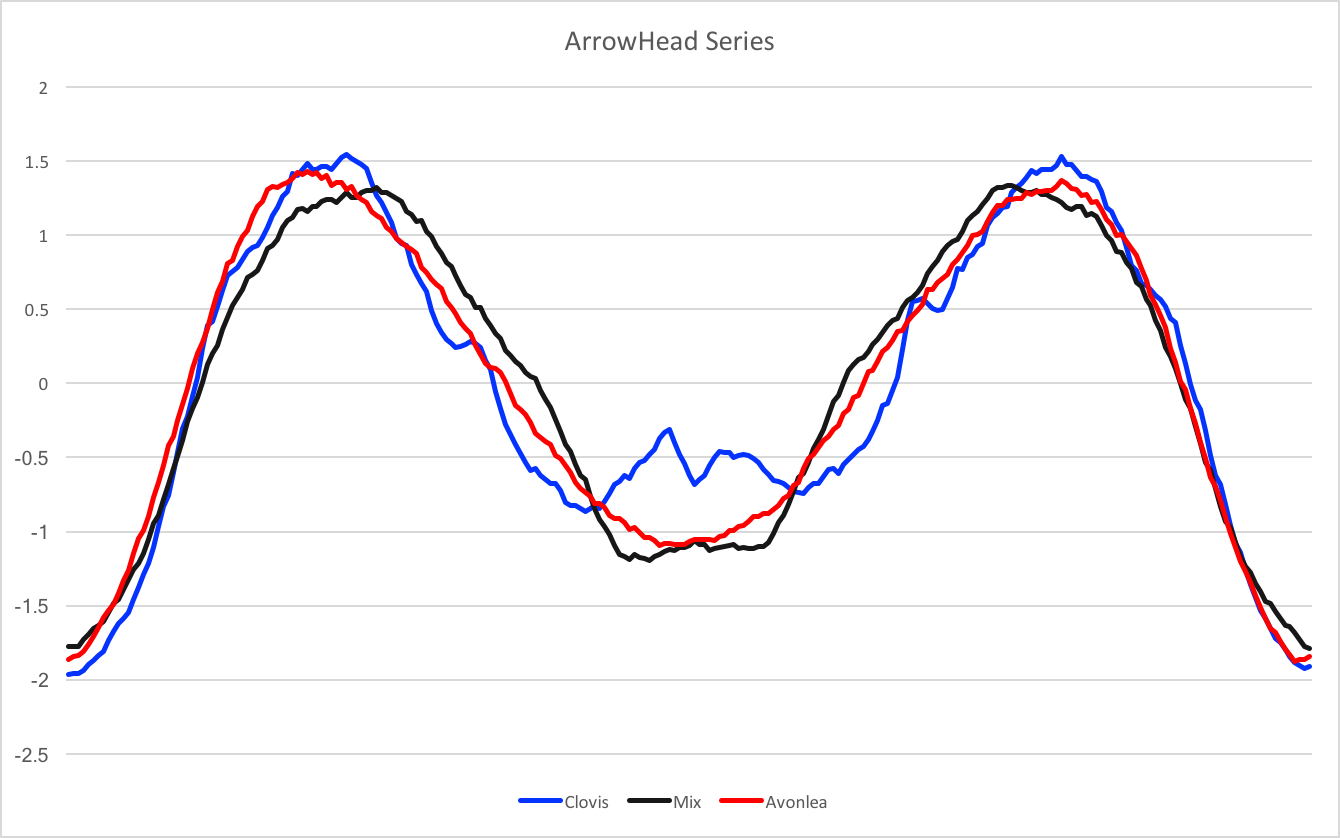
\includegraphics[width=130mm]{ArrowHead_Graph.png}
		\caption{Đầu mũi tên được biểu diễn dưới dạng Timeseries} 
		\label{ArrowHead_Graph.png}
	\end{center}
\end{figure}
\subsection{Bộ dữ liệu BeetleFly}
BeetleFly là bộ dữ liệu chuỗi thời gian được chuyển đổi từ đường viền hình ảnh của con bọ cánh cứng (Beetle) và con ruồi (Fly), được minh hoạ ở hình \ref{BeetleFly.png}.
Bộ dữ liệu này có 2 lớp là Beetle và Fly mỗi lớp có 20 phần tử, mỗi phần tử có 512 điểm dữ liệu.
\begin{figure}[!htbp]
	\begin{center}
		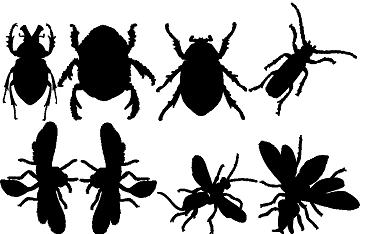
\includegraphics[width=130mm]{BeetleFly.png}
		\caption{Một số hình ảnh minh hoạ bộ dữ liệu BeetleFly} 
		\label{BeetleFly.png}
	\end{center}
\end{figure}
\subsection{Bộ dữ liệu Gun Point}
Bộ dữ liệu này là từ một video cảnh giác. Bộ dữ liệu gồm hai lớp, mỗi lớp gồm 100 mẫu. Tất cả các mẫu đều được tạo ra từ một diễn viên nữ và một diễn viên nam diễn xuất trong một phân cảnh.  Hai lớp bao gồm:
\begin{itemize}
\item Rút súng (Gun-Draw): Các diễn viên để tay ngang hông. Họ rút một khẩu súng từ túi da đeo ngang hông và chỉa súng về một đối tượng ở phía trước trong khoảng một giây, rồi đút súng lại vào túi da và để hai tay ngang hông. Hình \ref{GunPoint.png} là một minh họa về hình ảnh trích từ video này.
\item Chỉ (Point): Các diễn viên để tay ngang hông. Họ dùng ngón tay trỏ chỉ về một đối tượng ở phía trước trong khoảng một giây, rồi thu tay về để ngang hông.
Trong cả hai lớp, trung tâm của tay phải được theo dõi theo cả hai trục X và Y; tuy nhiên trong bộ dữ liệu này chỉ tập trung xem xét chuyển động theo trục X cho đơn giản.
\end{itemize}

\begin{figure}[!h]
	\begin{center}
		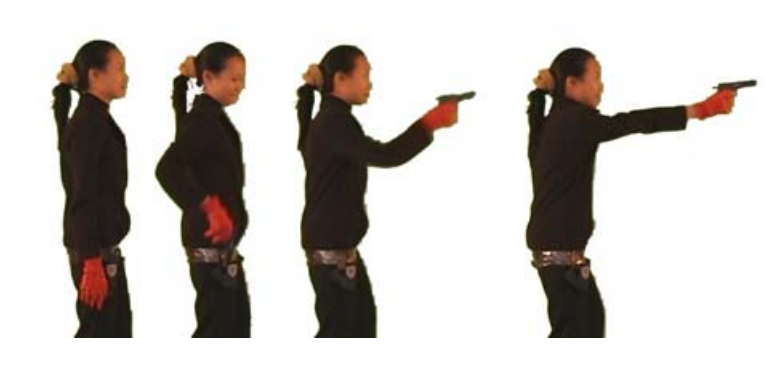
\includegraphics[width=130mm]{GunPoint.png}
		\caption{Vài ảnh rời trích từ video Gun-Draw: theo dõi hành vi của tay phải và chuyển thành một chuỗi cử động} 
		\label{GunPoint.png}
	\end{center}
\end{figure}
Toàn bộ chuyển động của hai lớp đều khá tương tự nhau. Tuy nhiên con người vốn có khả năng quan sát bằng mắt và phân biệt hai lớp hành vi một cách khá chính xác. Sự khác biệt tế nhị giữa hai lớp được diễn tả bằng hai đường cong đại diện cho hai lớp như trong hình \ref{Gun_Point_Graph.png}
\begin{figure}[!h]
	\begin{center}
		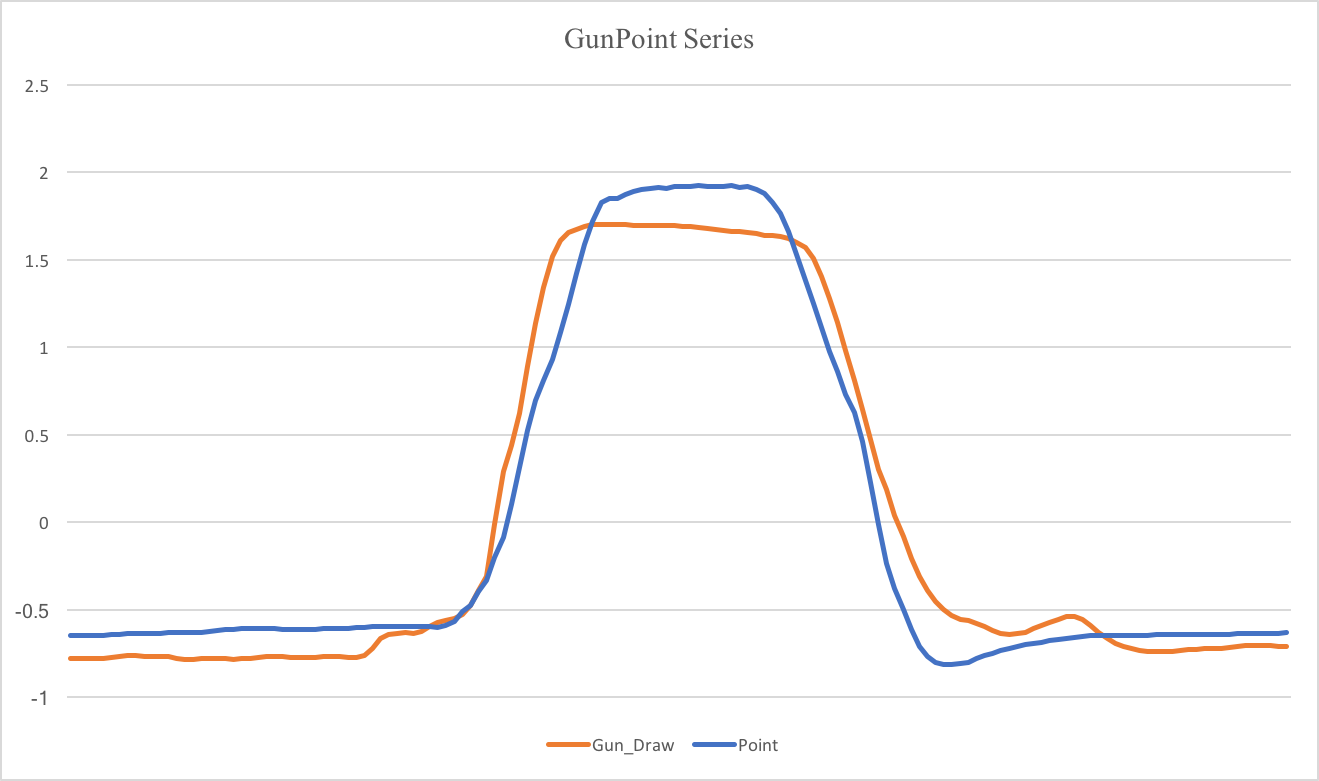
\includegraphics[width=130mm]{Gun_Point_Graph.png}
		\caption{Dạng chuỗi thời gian thuộc lớp Point và dạng chuỗi thời gian thuộc lớp Gun-Draw} 
		\label{Gun_Point_Graph.png}
	\end{center}
\end{figure}

Bộ dữ liệu này gồm 200 mẫu, mỗi lớp có 100 mẫu.
Tất cả các mẫu đều có cùng chiều dài là 150 điểm dữ liệu.
\subsection{Bộ dữ liệu Fish}
Bộ dữ liệu này là từ những hình ảnh của cá được chụp trong các video. Từ hình thù của từng con cá, hệ thống xử lý ảnh sẽ chuyển hình dạng hai chiều của cá thành một chuỗi thời gian đơn biến, như được minh họa trong hình \ref{Fish.png}.
\begin{figure}[H]
	\begin{center}
		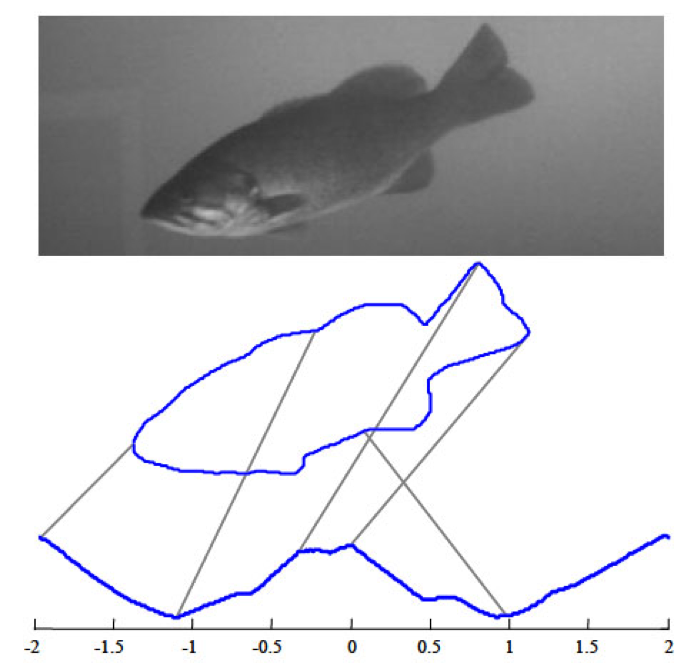
\includegraphics[width=130mm]{Fish.png}
		\caption{Chuỗi thời gian được tạo ra từ ánh xạ đường biên hình con cá} 
		\label{Fish.png}
	\end{center}
\end{figure}
Từ một tập hợp hình ảnh của nhiều con cá dưới dạng thức chuỗi thời gian đơn biến, chúng ta cần phân lớp chúng thành ra 7 loại cá có tên như sau: Chinook Salmon, Winter Coho, Brown Trout, Bonneville Cutthroat, Colorado River Cutthroat, Yellowstone Cutthroat, và Mountain Whitefish. \\
Bộ dữ liệu Fish này gồm có 350 chuỗi thời gian biểu diễn hình dạng đường biên của cá. Mỗi chuỗi thời gian có cùng chiều dài gồm 463 điểm dữ liệu. 
Chúng ta cần phân lớp bộ dữ liệu thành 7 lớp ứng với 7 loại cá có tên nêu trên.
\subsection{Bộ dữ liệu Trace}
Bộ dữ liệu này là một tập con của bộ dữ liệu Transient Classification Benchmark (dự án Trace). Đây là một bộ dữ liệu tổng hợp được thiết kế để mô phỏng sự hỏng hóc của thiết bị đo trong một nhà máy năng lượng hạt nhân. Bộ dữ liệu được tạo ra bởi Davide Roverso. Bộ dữ liệu đầy đủ gồm 16 lớp, 50 mẫu trong mỗi lớp. Mỗi mẫu gồm 4 đặc trưng. \\
Để đơn giản, bộ dữ liệu Trace ở đây chỉ gồm đặc trưng thứ hai của lớp 2 và 6 cùng đặc trưng thứ ba của lớp 3 và 7. Bộ dữ liệu Trace ở đây gồm 200 mẫu, 50 mẫu cho mỗi lớp. Tất cả các mẫu được nội suy để đưa về cùng chiều dài gồm 275 điểm dữ liệu.
Hình \ref{Trace_Graph.png} biểu diễn các lớp trong bộ dữ liệu Trace.
\begin{figure}[H]
	\begin{center}
		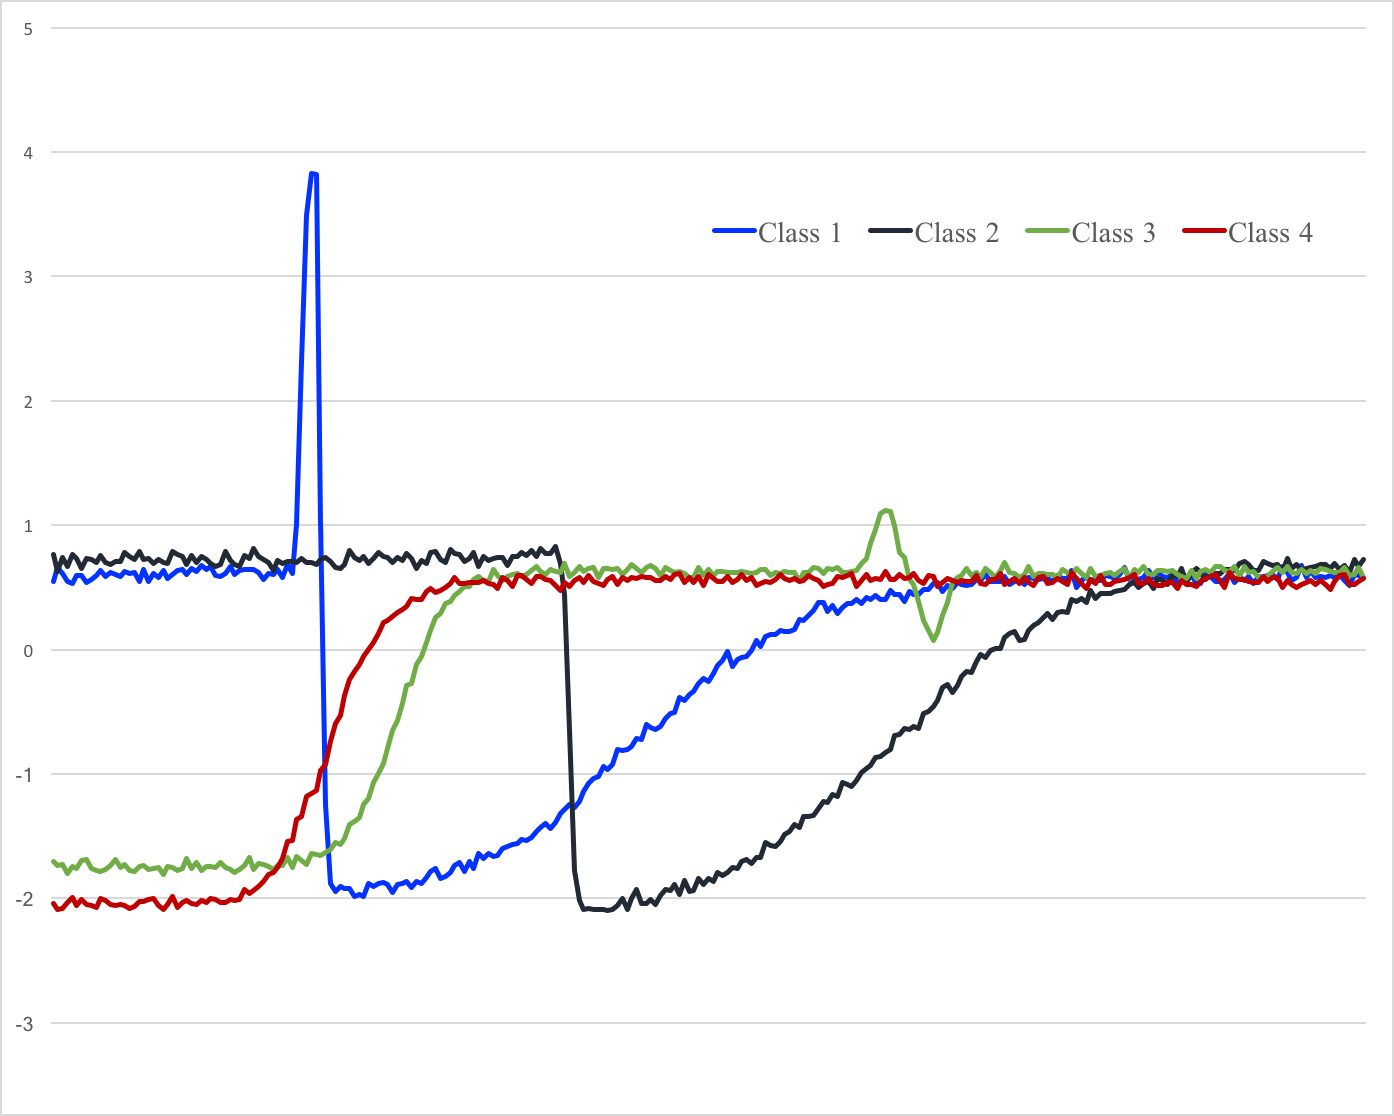
\includegraphics[width=130mm]{Trace_Graph.png}
		\caption{Biểu đồ biểu diễn các lớp trong bộ dữ liệu Trace} 
		\label{Trace_Graph.png}
	\end{center}
\end{figure}
\section{THỰC NGHIỆM SO SÁNH ĐỘ CHÍNH XÁC PHÂN LỚP TRƯỚC VÀ SAU KHI THU GỌN TẬP HUẤN LUYỆN}
Kết quả thực nghiệm cho thấy rằng, phân lớp k-NN dựa trên tập huấn đã thu gọn bằng kỹ thuật thu gọn RHC cho độ chính xác trung  thấp hơn khoảng $7\%$ so với độ chính xác phân lớp k-NN dựa trên tập huấn luyện ban đầu.
Nhưng thời gian thực hiện phân lớp trên tập huấn luyện đã thu gọn chỉ bằng khoảng $25\%$ so với thời gian thực hiện phân lớp trên tập huấn luyện ban đầu.

Độ chính xác phân lớp sau khi thu gọn với kỹ thuận RHC cao hơn hẵn (trung bình $22\%$) so với kỹ thuật Naive Ranking.

Bảng \ref{tab:classificationresult} trình bày chi tiết kết quả gọn tập huấn luyện và độ chính xác phân lớp trước thu gọn và sau khi thu gọn áp dụng các kỹ thuật thu gọn tập huấn luyện RHC và Naive Ranking.
\begin{table}[!htb]
\centering
    \begin{tabular}{| c | l | c | c |}
    \hline
	STT & Tên Tập Dữ Liệu & Độ Chính Xác Cao Nhất (\%) & Kích Thước Cửa Sổ Xoắn (\%)\\ \hline
    \rownumber  & ArrowHead & 79.4& 1\\ \hline
	\rownumber  & Beef & 63.3& 1\\ \hline
	\rownumber  & BeetleFly & 75.0& 2\\ \hline
	\rownumber  & BirdChicken & 75.0& 4\\ \hline
	\rownumber  & CBF & 100.0& 17\\ \hline
	\rownumber  & Car & 78.3& 7\\ \hline
	\rownumber  & Coffee & 96.4& 2\\ \hline
	\rownumber  & DiatomSizeReduction & 96.1& 14\\ \hline
	\rownumber  & FISH & 87.4& 5\\ \hline
	\rownumber  & Gun\_Point & 97.3& 2\\ \hline
	\rownumber  & Lighting2 & 88.5& 2\\ \hline
	\rownumber  & Lighting7 & 78.1& 3\\ \hline
	\rownumber  & Meat & 93.3& 1\\ \hline
	\rownumber  & Plane & 100.0& 4\\ \hline
	\rownumber  & Trace & 99.0& 4\\ \hline
    \end{tabular}
    \caption{Thông tin các tập dữ liệu thực nghiệm}\label{tab:dataset}
\end{table}
\begin{table}[!htb]
\centering
    \begin{tabular}{| l | c | c | c | c | c | c | c |}
    \hline
	\multirow{2}{*}{Bộ dữ liệu} & \multicolumn{3}{c|}{Tập huấn luyện}& \multicolumn{3}{c|}{Độ chính xác phân lớp KNN(\%)}\\
	\cline{2-7}
    & Ban đầu & Thu gọn & Tỉ lệ(\%) & Tập gốc &  RHC &Naive Rank\\
	\hline
	ArrowHead & 36 & 10 & 27.8 & 68.0 & \textbf{62.3} & 60.0\\ \hline
	Beef & 30 & 18 & 60.0 & 56.7 & \textbf{63.3} & 36.7\\ \hline
	BeetleFly & 20 & 5 & 25.0 & 70.0 & 60.0 & \textbf{70.0}\\ \hline
	BirdChicken & 20 & 8 & 40.0 & 75.0 & 60.0 & \textbf{65.0}\\ \hline
	Car & 60 & 18 & 30.0 & 75.0 & 40.0 & \textbf{56.7}\\ \hline
	CBF & 30 & 7 & 23.3 & 100.0 & 91.3 & \textbf{92.4}\\ \hline
	Coffee & 28 & 2 & 7.1 & 96.4 & \textbf{92.9} & 46.4\\ \hline
	DiatomSizeReduction & 16 & 4 & 25.0 & 96.1 & \textbf{80.4} & 40.5\\ \hline
	FISH & 175 & 47 & 26.9 & 86.3 & \textbf{70.3} & 62.9\\ \hline
	Gun\_Point & 50 & 7 & 14.0 & 88.0 & \textbf{69.3} & 60.0\\ \hline
	Lighting2 & 60 & 9 & 15.0 & 80.3 & \textbf{75.4} & 68.9\\ \hline
	Lighting7 & 70 & 23 & 32.9 & 75.3 & 61.6 & \textbf{64.4}\\ \hline
	Meat & 60 & 5 & 8.3 & 93.3 & \textbf{95.0} & 33.3\\ \hline
	Plane & 105 & 9 & 8.6 & 100.0 & \textbf{99.0} & 79.0\\ \hline
	Trace & 100 & 30 & 30.0 & 99.0 & \textbf{98.0} & 97.0\\ \hline
	\multicolumn{3}{|c|}{\textbf{Trung bình}} & \textbf{24.9} & \textbf{84.0} & \textbf{74.6} & \textbf{62.2} \\ \hline
    \end{tabular}
    \caption{So sánh độ chính xác phân lớp sau khi thu gọn tập huấn luyện bằng kỹ thuật RHC và kỹ thuật Naive Ranking}\label{tab:classificationresult}
\end{table}

\begin{table}[!htb]
\centering
    \begin{tabular}{| l | c | c | c | c | c | c | c |}
    \hline
	\multirow{2}{*}{Bộ dữ liệu} & \multicolumn{3}{c|}{Tập huấn luyện}& \multicolumn{3}{c|}{Độ chính xác phân lớp KNN(\%)}\\
	\cline{2-7}
    & Ban đầu & Thu gọn & Tỉ lệ(\%) & Tập gốc &  RHC &Naive Rank\\
	\hline
ArrowHead & 36 & 10 & 27.8 & 74.9 & \textbf{66.3} & 49.1\\ \hline
Beef & 30 & 18 & 60.0 & 56.7 & \textbf{63.3} & 36.7\\ \hline
BeetleFly & 20 & 5 & 25.0 & 65.0 & \textbf{70.0} & 50.0\\ \hline
BirdChicken & 20 & 8 & 40.0 & 75.0 & \textbf{65.0} & 60.0\\ \hline
Car & 60 & 18 & 30.0 & 76.7 & 61.7 & \textbf{73.3}\\ \hline
CBF & 30 & 7 & 23.3 & 98.8 & \textbf{96.3} & 68.0\\ \hline
Coffee & 28 & 2 & 7.1 & 96.4 & \textbf{92.9} & 46.4\\ \hline
DiatomSizeReduction & 16 & 4 & 25.0 & 95.8 & \textbf{80.1} & 40.5\\ \hline
FISH & 175 & 47 & 26.9 & 86.9 & \textbf{77.1} & 56.0\\ \hline
Gun\_Point & 50 & 7 & 14.0 & 96.7 & \textbf{94.0} & 73.3\\ \hline
Lighting2 & 60 & 9 & 15.0 & 86.9 & \textbf{75.4} & 52.5\\ \hline
Lighting7 & 70 & 23 & 32.9 & 76.7 & \textbf{67.1} & 58.9\\ \hline
Meat & 60 & 5 & 8.3 & 93.3 & \textbf{93.3} & 33.3\\ \hline
Plane & 105 & 9 & 8.6 & 100.0 & \textbf{96.2} & 78.1\\ \hline
Trace & 100 & 30 & 30.0 & 99.0 & \textbf{96.0} & 91.0\\ \hline
\multicolumn{3}{|c|}{\textbf{Trung bình}} & \textbf{24.9} & \textbf{85.3} & \textbf{79.6} & \textbf{57.8}\\ \hline
    \end{tabular}
    \caption{So sánh độ chính xác phân lớp sau khi thu gọn tập huấn luyện bằng kỹ thuật RHC và kỹ thuật Naive Ranking}\label{tab:classificationresult}
\end{table}

\begin{table}[!htb]
\centering
    \begin{tabular}{| l | c | c | c | c | c | c | c |}
    \hline
	\multirow{2}{*}{Bộ dữ liệu} & \multicolumn{3}{c|}{Tập huấn luyện}& \multicolumn{3}{c|}{Độ chính xác phân lớp KNN(\%)}\\
	\cline{2-7}
    & Ban đầu & Thu gọn & Tỉ lệ(\%) & Tập gốc &  RHC &Naive Rank\\
	\hline
ArrowHead & 36 & 10 & 27.8 & 79.4 & \textbf{77.7} & 46.3\\ \hline
Beef & 30 & 18 & 60.0 & 63.3 & \textbf{73.3} & 46.7\\ \hline
BeetleFly & 20 & 5 & 25.0 & 75.0 & \textbf{75.0} & 45.0\\ \hline
BirdChicken & 20 & 8 & 40.0 & 75.0 & \textbf{65.0} & 60.0\\ \hline
Car & 60 & 18 & 30.0 & 78.3 & 51.7 & \textbf{71.7}\\ \hline
CBF & 30 & 7 & 23.3 & 100.0 & \textbf{96.7} & 77.0\\ \hline
Coffee & 28 & 2 & 7.1 & 96.4 & \textbf{92.9} & 46.4\\ \hline
DiatomSizeReduction & 16 & 4 & 25.0 & 96.1 & \textbf{80.4} & 40.5\\ \hline
FISH & 175 & 47 & 26.9 & 87.4 & \textbf{74.3} & 55.4\\ \hline
Gun\_Point & 50 & 7 & 14.0 & 97.3 & \textbf{94.0} & 70.7\\ \hline
Lighting2 & 60 & 9 & 15.0 & 88.5 & \textbf{73.8} & 47.5\\ \hline
Lighting7 & 70 & 23 & 32.9 & 78.1 & \textbf{67.1} & 57.5\\ \hline
Meat & 60 & 5 & 8.3 & 93.3 & \textbf{91.7} & 33.3\\ \hline
Plane & 105 & 9 & 8.6 & 100.0 & \textbf{96.2} & 78.1\\ \hline
Trace & 100 & 30 & 30.0 & 99.0 & \textbf{96.0} & 91.0\\ \hline
\multicolumn{3}{|c|}{\textbf{Trung bình}} & \textbf{24.9} & \textbf{87.1} & \textbf{80.4} & \textbf{57.8}\\ \hline
    \end{tabular}
    \caption{So sánh độ chính xác phân lớp sau khi thu gọn tập huấn luyện bằng kỹ thuật RHC và kỹ thuật Naive Ranking}\label{tab:classificationresult}
\end{table}
%%%%%%%%%%%%%%%%%%%%%%%%%%%%%%%%%
\newpage
\begin{spacing}{1.0}
\begin{thebibliography}{99}
\bibitem{Buza}\label{Buza}
Buza, K., Nanopoulos A., and Schmidt-Thieme L. (2011), 
"INSIGHT: Efficient and Effective Instance Selection for Time-Series  Classification", Proceedings of PAKDD 2011, Shenzen, China, May 24-27.
\bibitem{CJA}\label{CJA}Chen, C.H., Jozwik, A. (1996), "A sample set condensation algorithm for the class sensitive artificial neural network. Pattern Recogn". Lett. 17(8), 819–823.
\bibitem{UCR}\label{UCR}Chen, Y., Keogh, E., Ha, B., Begum, N. Bagnall, A., Mueen, A. and Batista, G.: The UCR Time Series Classification Archive, URL: \url{http://www.cs.ucr.edu/~eamonn/time_series_data/}
\bibitem{Duong Tuan Anh}\label{Duong Tuan Anh}
Duong Tuan Anh (2009), “An Overview of Similarity Search in Time Series Data”, in Proceedings of the 11th Conference on Science and Technology -  Section of Computer Science and Engineering, Ho Chi Minh City University of Technology, 21-23 October, 2009, pp. 86-95.
\bibitem{E.keogh}\label{E.keogh}  Keogh E., (2002), 
"Exact indexing of dynamic time warping". In Proc.VLDB, Proceedings of the 28th VLDB Conference, Hong Kong, China.
\bibitem{E.keogh2}\label{E.keogh2}  Keogh E., Ratanamahatana C.,
"Three Myths about Dynamic Time Warping Data Mining".
\bibitem{Concepts and Techniques}\label{Concepts and Techniques} Han J., Kamber M., Pei J. (2012),
Data Mining: Concepts and Techniques, Third Edition, Morgan Kaufmann Publishers.
\bibitem{J. Lin}\label{J. Lin}Lin J., Keogh E., Lonardi S., and Chiu B. (2003), 
“A symbolic representation of time series, with implications for streaming algorithms”, in SIGMOD’03, 2003.
\bibitem{Hart}\label{Hart}Hart,P.E., "The condensed nearest neighbor rule. IEEE Transactions on Information Theory" 14(3), 515–516 (1968)
\bibitem{Stefanos Ougiaroglou}\label{Stefanos Ougiaroglou}  Ougiaroglou S. and Evangelidis G. (2016), 
"RHC: a non-parametric cluster-based data reduction for efficient k-NN classification". Pattern Analysis and Applications, Vol 19, 93-109
\bibitem{Stefanos Ougiaroglou Prototype}\label{Stefanos Ougiaroglou Prototype} Ougiaroglou S., Karamitopoulos L., Tatoglou C. (2015),
"Applying Prototype Selection and Abstraction Algorithms for Efficient Time-Series
Classification". Artificial Neural Networks Methods and Applications in Bio-/Neuroinformatics pp.333-348
\bibitem{SakoeChiba}\label{SakoeChiba}Sakoe, H. and Chiba, S. (1978), Dynamic programming algorithm optimization for spoken word recognition. In IEEE Transactions on Acoustics, Speech, and Signal Processing, Vol. 26, pp. 43-49.
\bibitem{RSP}\label{RSP} Sánchez, J.S. (2004), "High training set size reduction by space partitioning and prototype ab straction". Pattern Recognition 37(7), 1561–1564
\bibitem{Decision tree}\label{Decision tree} Yamada, Y., Suzuki, E., Yokoi H., Takabayashi K. (2003),
"Decision-tree induction from time-series data based on a standard-example split test". In: Proc. Twentieth International Conference on Machine Learning (ICML), pp. 840–847
\bibitem{Xi}\label{Xi} Xi X., Keogh E., Shelton C., Wei L., and Ratanamahatana C. A. 
(2006), “Fast Time Series
Classification using Numerosity Reduction.” In the Proc of the 23rd ICML, 1033-1040.
\bibitem{DMKSWang}\label{DMKSWang}Wang X., Mucen A., Ding H., Trjcevske G., Scheuermann P., Keogh E. (2013), "Experiment Comparision of Representation Methods and Distance Measures for Time Series, Data Mining and Knowledge Discovery", Vol. 26, pp.275-309.

\end{thebibliography}
\end{spacing}
\end{document}